\documentclass[12pt]{article}
\usepackage[T1]{fontenc}
\usepackage[utf8]{inputenc}
\usepackage[spanish]{babel}
\decimalpoint
\usepackage{graphicx}
\usepackage{amssymb} %Para usar el símbolo del conj. de los Reales.%
\usepackage{hyperref} % Siempre debe ser el último paquete.

\setlength{\parindent}{0em} %justificado%
\setlength{\parskip}{1em} %espacio entre párrafos%
\renewcommand{\baselinestretch}{1.15} %line-space%

\begin{document}

\title{Apuntes `Calculus 1A: Differentiation'}
\author{}
\date{}
\maketitle

\tableofcontents

\newpage

\section{Límites.}


\subsection{Moviéndonos más y más cerca.}

Cálculo es todo sobre \textbf{funciones}. Probablemente sabemos que si una función ``f'' toma como entrada (\textit{input}) a ``x'', entonces su salida (\textit{output}) será $f(x)$. Pero en cálculo no estamos interesados en observar una entrada y encontrar su salida, más bien queremos considerar un \textbf{rango enorme de entradas}, de manera que vamos a querer saber \textbf{qué ocurre cuando la entrada se ``mueve'' o ``varía''}.

Veamos el siguiente ejemplo.

\underline{Ejemplo}: ¿Qué ocurre cuando la entrada $x$ se mueve desde la izquierda y se va ubicando cada vez más cerca de $1$ (por mencionar un punto cualquiera)?

\underline{Respuesta}: Veamos el siguiente gráfico, para visualizar el problema que estamos tratando.

\begin{figure}[hbt!]
\centering
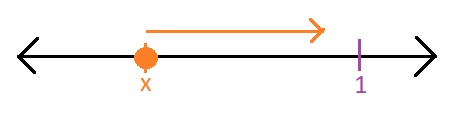
\includegraphics[scale=0.7]{img/moving_point.jpg}
\end{figure}

Vamos a denotar que ``$x$ se acerca mucho a $1$'' como $x \to 1$, lo cual no significa por ningún sentido que $x$ va a ser igual a 1 (i.e., $x \neq 1$). En otras palabras, solo vamos a considerar todos aquellos números que se acercan a 1.

Ahora bien, como $x$ se va a mover, eso quiere decir que su salida $f(x)$ también lo hará. Por lo tanto, surge una segunda pregunta.

\newpage

\underline{Ejemplo 2}: Si $x$ se mueve muy cerca a 1 desde la izquierda, ¿hacia qué punto se moverá $f(x)$?

Considere:
\[f(x) = \frac{\sqrt{3-5x+x^{2}+x^{3}}}{x-1}\]
\underline{Respuesta 2}: Lo que haremos a continuación es seleccionar ciertos valores que se encuentren a la izquierda\footnote{De hecho, si $x = 1$, entonces $f(x)$ se va a indeterminar debido a su denominador.} de 1 y los usaremos como entrada a la función $f(x)$.

Tomemos los siguientes valores\footnote{Pueden ser muchísimos más, pero para entender el ejemplo, usemos estos cuatro.}
\[x = \{0,\, 0.5,\, 0.9,\, 0.99\}\]
Ahora veamos a qué valor se acerca $f(x)$ con estos valores:

\begin{center}
\begin{tabular}{c | c}

$x$ & $f(x)$ \\
\hline
0 & $\approx$ -1.73\\
0.5 & $\approx$ -1.87\\
0.9 & $\approx$ -1.97\\
0.99 & $\approx$ -1.997\\

\end{tabular}
\end{center}

Como podemos apreciar, a medida que $x \to 1$ desde la izquierda, pareciera que $f(x) \to -2$.

Ahora veamos una tercera pregunta a partir de esta última.

\underline{Ejemplo 3}: Digamos que $x$ se acerca cada vez más a 1, pero \textbf{desde la derecha}. ¿Qué ocurrirá con $f(x)$? y ¿hacia qué valor se acerca?

\underline{Respuesta 3}: Al igual que antes, tomemos algunos valores de forma arbitaria que se acerquen a 1 desde la derecha, pero que sean menores a éste.
\[x = \{2,\, 1.5,\, 1.1,\, 1.01,\, 1.001\}\]
Veamos ahora cómo se comporta $f(x)$.

\begin{center}
\begin{tabular}{c | c}

$x$ & $f(x)$ \\
\hline
2 & 2.236068\\
1.5 & 2.12132\\
1.1 & 2.024846\\
1.01 & 2.002498\\
1.001 & 2.00025\\

\end{tabular}
\end{center}

Como podemos apreciar, a medida que $x \to 1$ desde la derecha, $f(x) \to 2$.


\subsection{Límites de un lado}

Cuando hablamos, por ejemplo, que $x$ se aproxima a 1 desde la izquierda, lo denotamos de la siguiente manera:
\[x \to 1^{-}\]
El signo ``negativo'' que está como exponente indica que el valor de $x$ viene desde la dirección negativa (izquierda) de, en este caso, 1. Por consiguiente, si viene desde la derecha:
\[x \to 1^{+}\]
Entonces, como dijimos en la sección anterior, cuando $x \to 1^{-}$, entonces $f(x) \to -2$.

Por otra parte, cuando $x\to 1^{+}$, entonces $f(x) \to 2$.

Grafiquemos la función $f(x)$ con los valores que hemos dado tanto desde la izquierda como desde la derecha\footnote{Quité los valores 0.99 y 1.001, porque o sino los puntos excluidos (bordes azules) no se iban a ver en el gráfico.}.

\begin{figure}[hbt!]
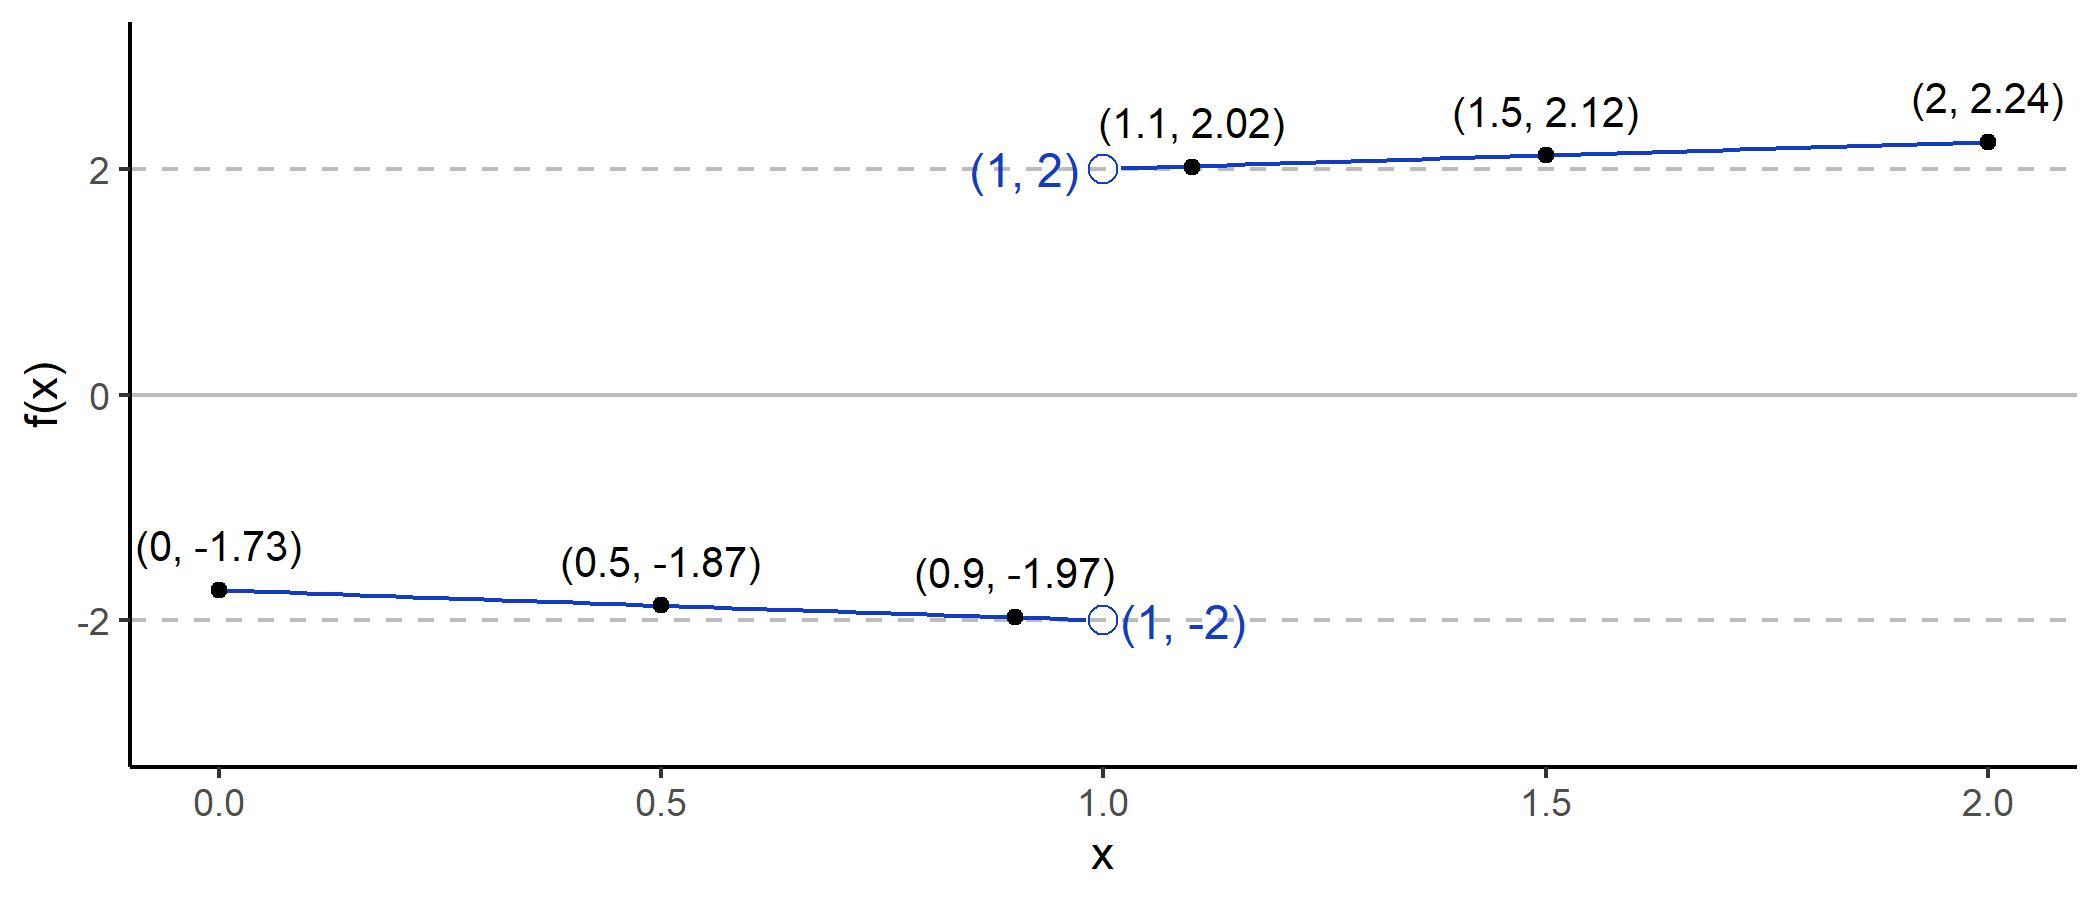
\includegraphics[scale=0.7]{img/limit_plot.jpg}
\end{figure}

Como se puede observar, hay 2 puntos que tienen sus bordes azules pero sin color adentro. Son los puntos (1, 2) y (1, -2) y están de esa manera porque, en realidad, no están incluidos en el gráfico. Recordemos que si $x = 1$, entonces $f(x)$ se indefine. Podemos entenderlo como un recordatorio de que, con ese valor de $x$, se indetermina $f(x)$ y por eso se ilustra como un círculo vacío (o una circunferencia).

\underline{Definición del límite}.

Con la información que manejamos, le daremos un nombre al fenómeno de que un valor se acerque a otro. Lo conoceremos de ahora en adelante como \textbf{Límite}.

Conceptualmente, por ejemplo, ahora vamos a decir que: ``El límite de $f(x)$ cuando $x \to 1^{+}$, es igual a 2''; y lo vamos a denotar de la siguiente manera:
\[\lim_{x \to 1^{+}} f(x) =  2\]
Al límite que tiende desde $x$ hasta un valor, desde la derecha (e.g., $\lim_{x \to 1^{+}}$), se le denomina como \textbf{Límite de la Derecha}.

Mientras que al límite que tiende desde $x$ hasta un valor desde la izquierda (e.g., $\lim_{x \to 1^{-}}$), se denomina como el \textbf{Límite de la Izquierda}. Un ejemplo es el siguiente:
\[\lim_{x \to 1^{-}} f(x) = -2\]
Tanto en el gráfico de arriba como en el que podemos apreciar a continuación, la curva de abajo corresponde al límite de la izquierda, mientras que la de arriba, es el límite de la derecha.

\begin{figure}[hbt!]
\centering
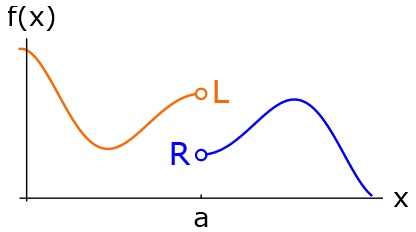
\includegraphics[scale=0.7]{img/limit_plot_2.jpg}
\end{figure}


\subsection{Posibles Comportamientos de los Límites.}

Los límites se pueden comportar de muchas maneras. En el caso que vimos en las dos secciones anteriores, los límites de la izquierda y la derecha de $f(x)$ no se acercaban a un mismo valor: en el primer caso ($\lim_{x \to 1^{-}}$), el límite fue igual a $-2$; mientras que en el segundo ($\lim_{x \to 1^{+}}$), fue igual a 2.

No obstante, puede darse el caso en que \textbf{ambos límites coincidan}. Veamos el siguiente ejemplo.

Sea:
\[g(x) = \frac{x}{tan(2x)}\]
Entonces:
\[\lim_{x \to 0^{\pm}} g(x) = ?\]
Construyamos una tabla tanto para $x \to 0^{-}$ como para $x \to 0^{+}$, en $g(x)$ y grafiquemos sus valores.

Partamos con el $lim_{x \to 0^{-}} g(x)$.

\begin{center}

\begin{tabular}{c | c}

x & g(x)\\
\hline
-1 & -0.4577\\
-0.5 & 0.3210\\
-0.1 & 0.4933\\
-0.05 & 0.4983\\
-0.01 & 0.4999\\

\end{tabular}

\end{center}

Ahora con el $lim_{x \to 0^{+}} g(x)$.

\begin{center}

\begin{tabular}{c | c}

x & g(x)\\
\hline
1 & -0.4577\\
0.5 & 0.3210\\
0.1 & 0.4933\\
0.05 & 0.4983\\
0.01 & 0.4999\\

\end{tabular}

\end{center}

Como podemos apreciar en ambas tablas, pareciera que tanto para $x \to 0^{-}$ como para $x \to 0^{+}$, el límite para ambos casos de $g(x)$ es igual a 0.5. Algo que también podemos ver en su gráfico.

\begin{figure}[hbt!]
\centering
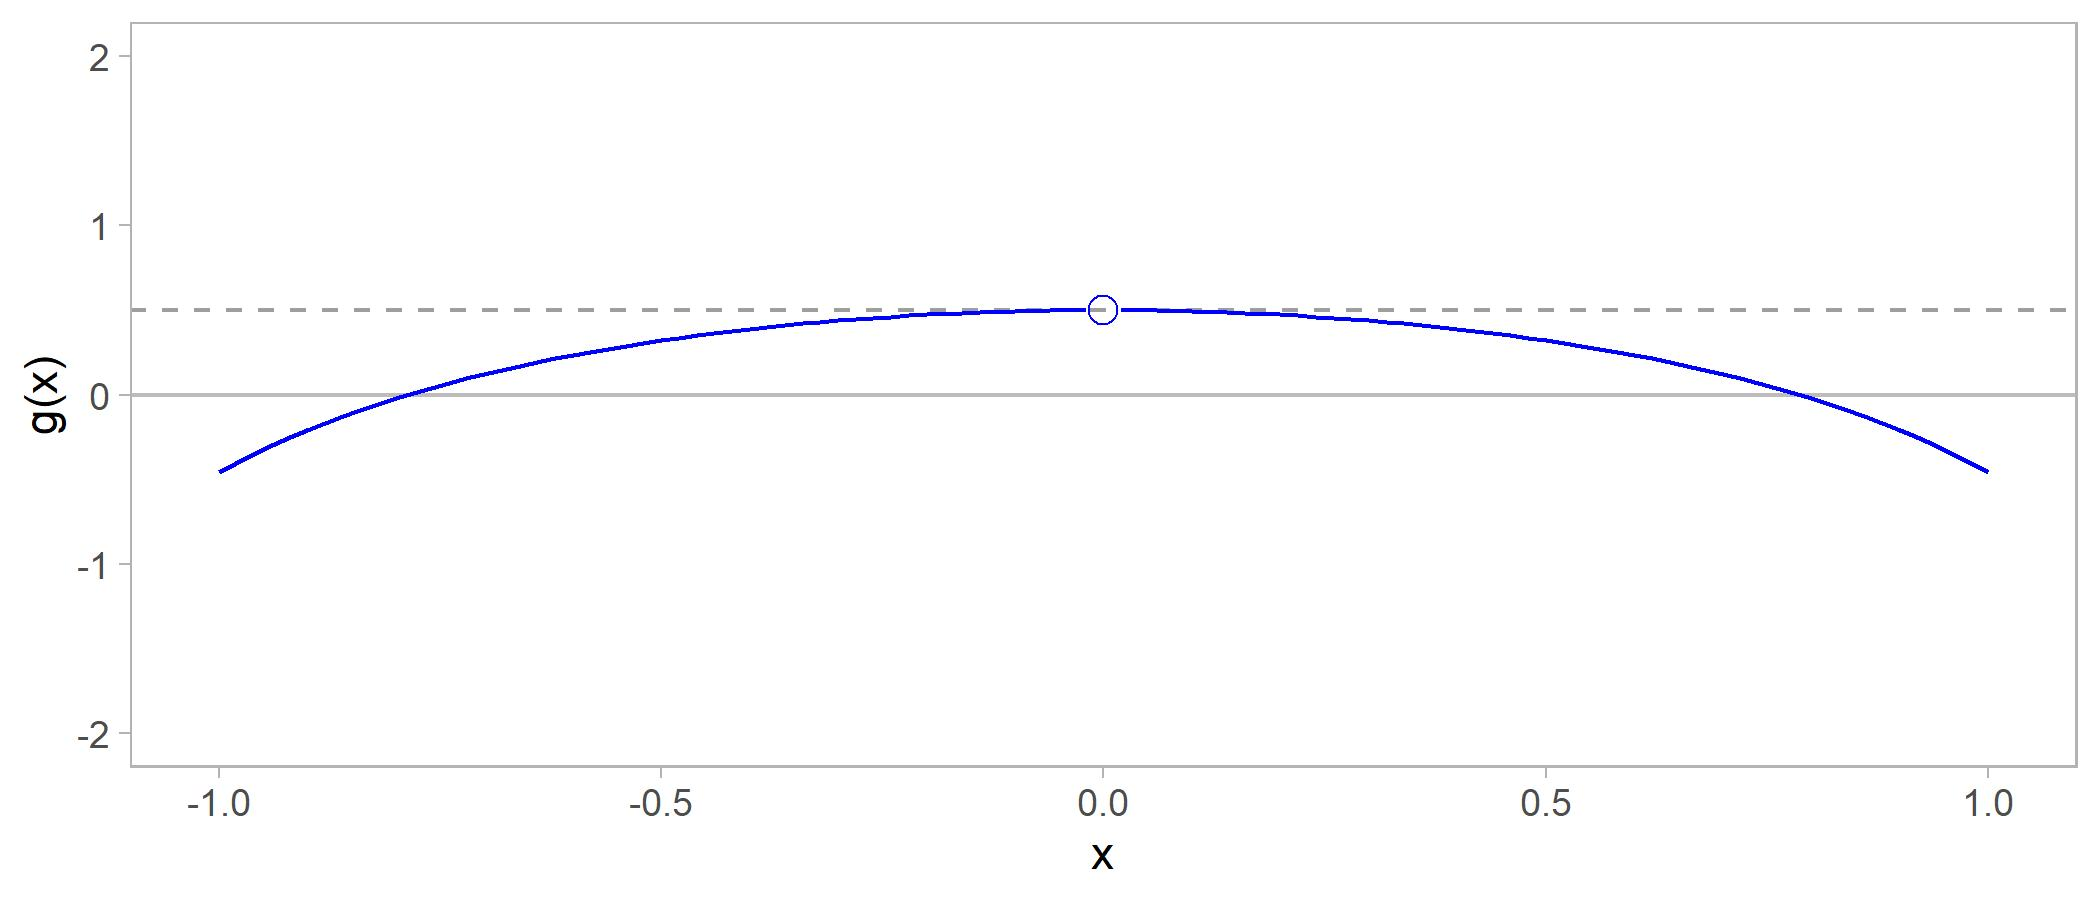
\includegraphics[scale=0.7]{img/limit_plot_g.jpg}
\end{figure}

Un segundo caso es que \textbf{uno de los límites no exista}.

Sea:
\[h(x) = \frac{|x| + sen(x)}{x^{2}}\]
Entonces:
\[\lim_{x \to 0^{\pm}}h(x)=?\]
Cuando el $\lim_{x \to 0^{-}}h(x)$:

\begin{center}

\begin{tabular}{c | c}

x & h(x)\\
\hline
-1 & 0.1585\\
-0.5 & 0.0823\\
-0.1 & 0.0167\\
-0.01 & 0.0017\\
-0.001 & 0.0002\\

\end{tabular}

\end{center}

Y cuando el $\lim_{x \to 0^{+}}h(x)$

\begin{center}

\begin{tabular}{c | c}

x & h(x)\\
\hline
1 & 1.8415\\
0.5 & 3.9177\\
0.1 & 19.9833\\
0.05 & 39.9917\\
0.01 & 199.9983\\

\end{tabular}

\end{center}

Como podemos observar en las últimas dos tablas, si bien en la primera es posible identificar que el $\lim_{x \to 0^{-}} h(x) = 0$, en el caso del $h(x)$ cuando $x \to 0^{+}$, esta función solo va haciéndose más y más grande, de manera que \textbf{su límite no está definido}. También podemos observarlo en su gráfico, en donde $h(x)$ cuando $x \to 0^{+}$ crece formando una asíntota vertical (línea segmentada).

%Por algún motivo, al enmarcarlo en \begin{figure}, etc, la imagen no se ubica donde debería, por eso no lo ocupo acá%
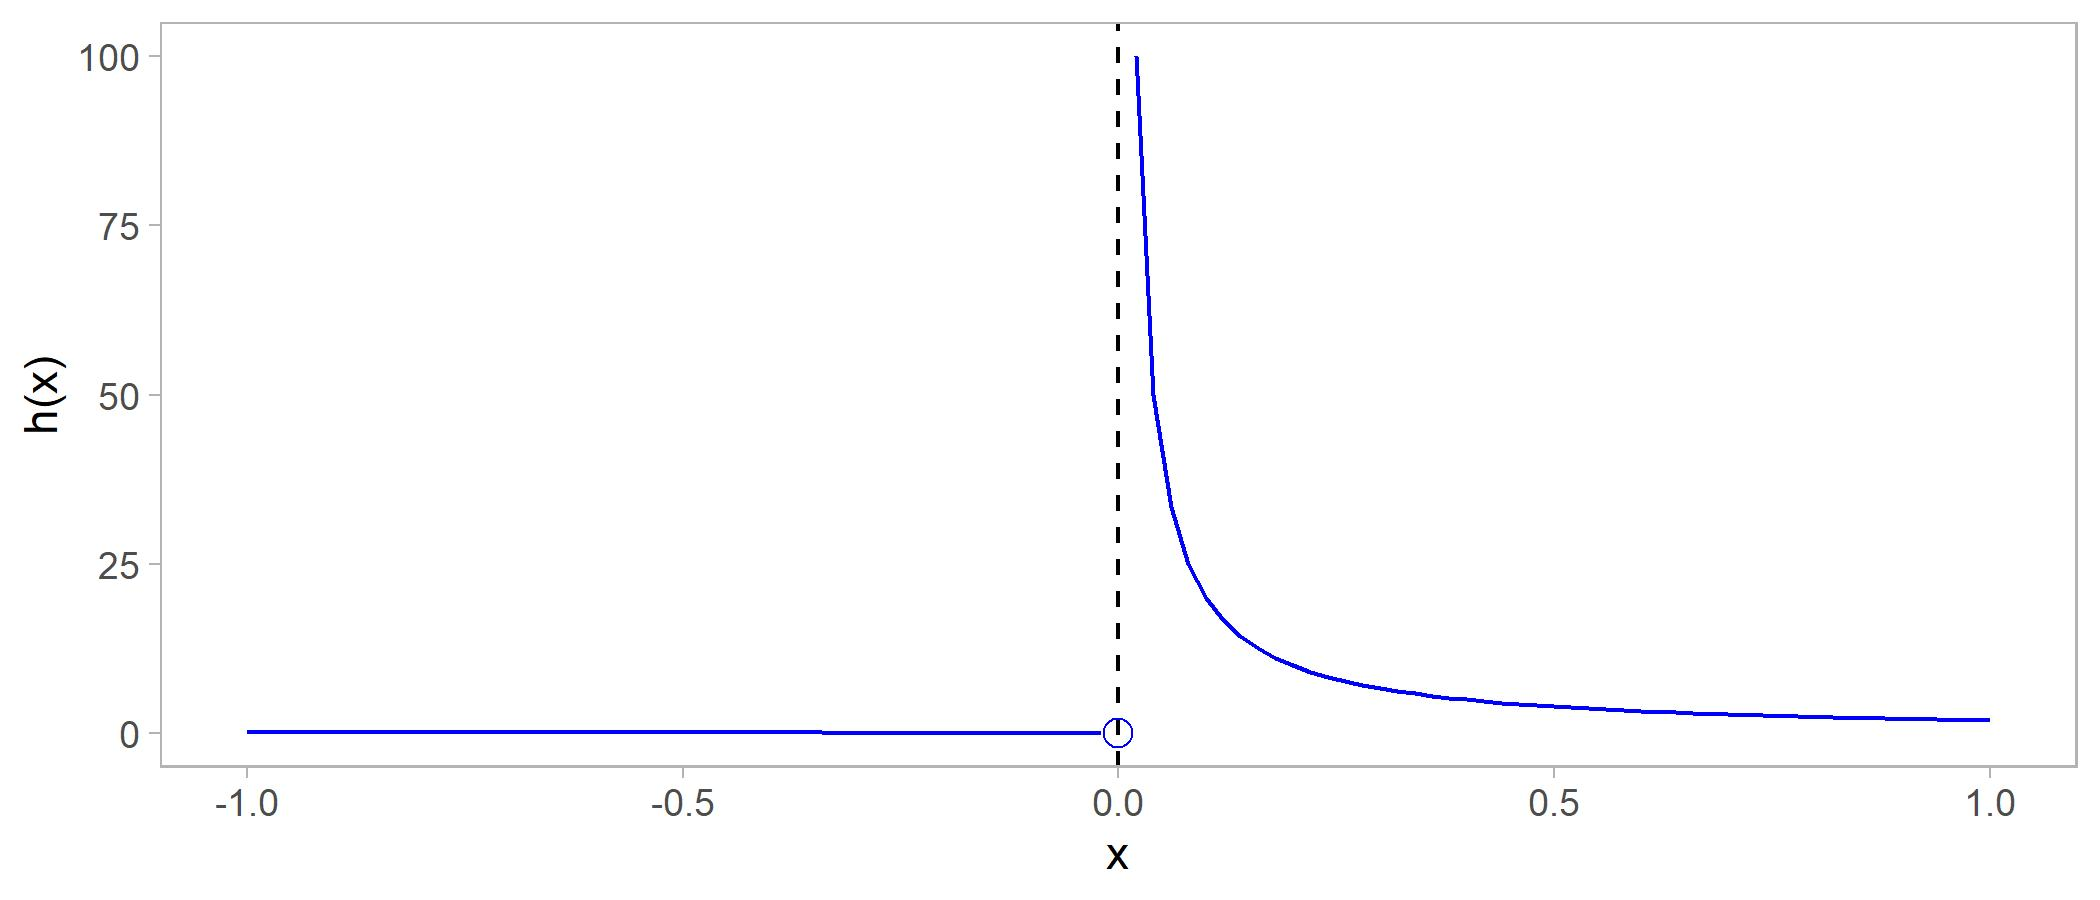
\includegraphics[scale=0.7]{img/limit_plot_h.jpg}

Finalmente, veamos la siguiente función, la cual cuando $x$ se acerca a cero, \textbf{su límite no se acerca a un valor en particular ni se hace más grande o más pequeña}.

Sea:
\[j(x) = sen (\frac{x}{13})\]
Entonces:
\[\lim_{x \to 0^{+}} j(x) = ?\]
En este caso, solo nos centraremos en el límite cuando $x \to 0^{+}$.

\begin{center}

\begin{tabular}{c | c}

x & h(x)\\
\hline
1 & 0.4202\\
0.5 & 0.7626\\
0.1 & -0.9301\\
0.05 & 0.6832\\
0.01 & -0.5805\\
0.005 & -0.9454\\

\end{tabular}

\end{center}

En esta tabla no es muy notorio (quizá tendríamos que agregar más valores a $x$), pero la función $h(x)$ se mueve entre 1 y -1, algo que se puede ver con mayor claridad en su gráfica de abajo. Probablemente esto se explica debido al comportamiento de la función $sen(x)$.

\begin{figure}[hbt!]
\centering
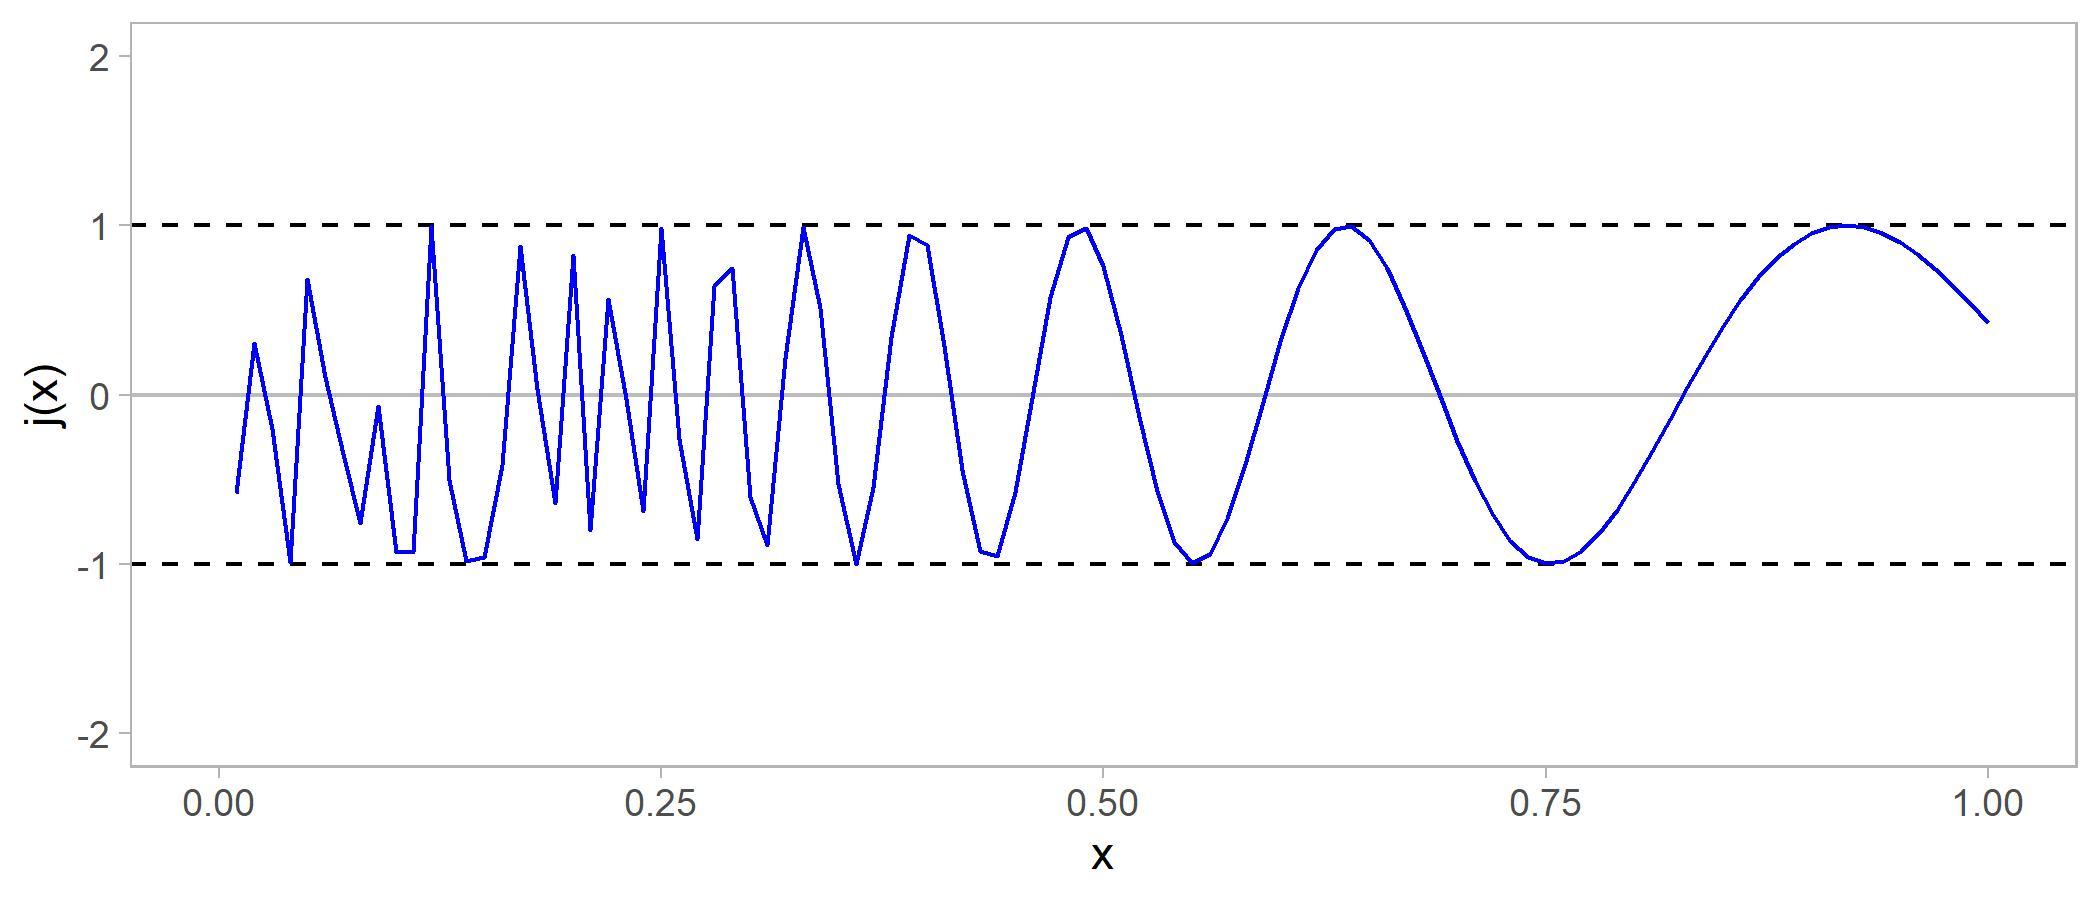
\includegraphics[scale=0.7]{img/limit_plot_j.jpg}
\end{figure}

Por otra parte, es claro que el $\lim_{x \to 0^{+}} h(x)$ \textbf{no está definido}.


\subsection{El Límite General.}

Hasta ahora ya hemos aprendido tanto del límite de la izquierda (valores de $x$ que son cercanos a un número, desde la izquierda) como el límite de la derecha (valores de $x$ que son cercanos a un número, desde la derecha).

No obstante, en muchas ocasiones vamos a querer saber qué valores de $x$ son cercanos a un número, sin las restricciones que hemos visto hasta ahora. A este caso se le denomina como \textbf{el límite general} y se denota de la siguiente manera:
\[\lim_{x \to a} f(x) = L\]
En primer lugar, ahora $a$ no tiene un $+$ o $-$ como exponente.

Este límite se puede leer como: ``Si cada vez que $x$ se acerca a $a$ desde cualquier lado (der. o izq.), $f(x)$ se hará más y más cercano a $L$''.

En otras palabras, \textbf{el límite general será igual a $L$} cuando tanto \textbf{el límite de la izquierda y el de la derecha sean iguales}. Es decir:
\[\lim_{x \to a} f(x) = L \iff \lim_{x \to a^{-}} f(x) = \lim_{x \to a^{+}} f(x) = L\]

En un gráfico, se vería más o menos de la siguiente manera:

\begin{figure}[hbt]
\centering
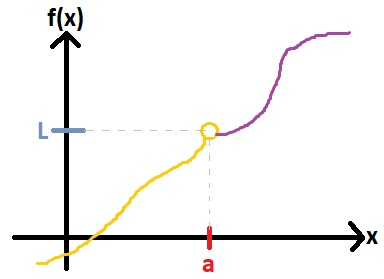
\includegraphics[scale=0.7]{img/overall_limit.jpg}
\end{figure}

También podemos denotarlo como: ``$f(x) \to L$ a medida que $x \to a$''.

Solo no olvidemos que los límites solo se preocupan por los valores de $x$ que se acercan a $a$ (i.e., $x \to a$) y NO por los que son iguales a $a$ (i.e., $x \neq a$). En ese sentido, el círculo vacío (a, L) que pusimos en el gráfico de arriba, podemos ubicarlo ahí, arriba, abajo o no tener uno si $f(a)$ no existe, ya que no va a afectar al límite. Otra vez, el valor del límite de $f(x)$ es el valor de $x \to a$, no el que es igual a $a$.

Ahora bien, ¿podría no existir un límite general? Sí. Una forma es que \textbf{no exista el límite en uno de los lados}.

Por ejemplo, $\lim_{x \to a^{+}}f(x) = L$, pero $\lim_{x \to a^{-}}f(x) = -\infty$.

\begin{figure}[hbt]
\centering
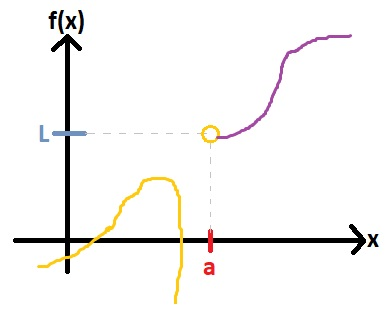
\includegraphics[scale=0.6]{img/overall_limit_2.jpg}
\end{figure}

Otra forma en que podría no existir un límite general es que \textbf{tanto el límite de la derecha como el de la izquierda existan, pero \underline{no sean iguales}}.

\begin{figure}[hbt]
\centering
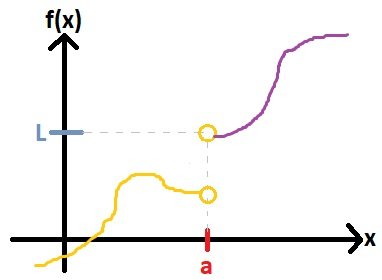
\includegraphics[scale=0.7]{img/overall_limit_3.jpg}
\end{figure}

Como se mencionó anteriormente, el límite de la izquierda y de la derecha de $f(x)$ deben \textbf{existir y ser iguales} para que exista el límite general de $f(x)$.

De ahora en adelante solo nos referiremos al ``límite general'' simplemente como ``límite'', sin especificar si es de la derecha o de la izquierda. Y esta idea del límite es la base para el Cálculo en su conjunto.


\subsection{Leyes de los Límites.}

Hasta ahora hemos visto el límite de una función en un punto en particular. En esta ocasión, aprenderemos sobre qué podemos hacer si conocemos el límite de múltiples funciones, \textbf{en un mismo punto}.

Por ejemplo, digamos que tenemos los límites de las funciones $f(x)$ y $g(x)$, en donde respectivamente son iguales a 5 y 3; y en ambas $x \to a$. Es decir:
\[\lim_{x \to a}f(x)=5 \, y \, \lim_{x \to a} g(x) = 3\]
Ahora hagamos una combinación de funciones, en donde sumemos estas dos y, luego, podemos buscar el límite de la suma de estas dos funciones, en un punto dado.
\[\lim_{x \to a}[(f + g)(x)]\]
\[\lim_{x \to a}[f(x) + g(x)]\]
Este límite será igual a la suma de los límites de las funciones $f(x)$ y $g(x)$, en donde en ambos $x \to a$.
\[\lim_{x \to a}[f(x) + g(x)] = \lim_{x \to a}f(x) + \lim_{x \to a}g(x)\]
\[\lim_{x \to a}[f(x) + g(x)] = 5 + 3\]
\[\lim_{x \to a}[f(x) + g(x)] = 8\]
Ahora justifiquemos lo que acabamos de hacer. 

Estamos viendo qué ocurre cuando $x \to a$. Sabemos que $f(x) \to 5$, lo cual no significa que $f(x) = 5$, pero se aleja por una pequeña cantidad de error. De manera que podemos escribir que $f(x)$ es igual a $5$ más el pequeño error, que denotaremos con la letra griega $\varepsilon$ (épsilon)\footnote{Los índices 1 y 2 en $\varepsilon$, son solo para diferenciarlos.}:
\[f(x) = 5 + \varepsilon_{1}\]
Lo anterior también lo podemos aplicar a $g(x)$:
\[g(x) = 3 + \varepsilon_{2}\]
Ahora bien, como dijimos, $\varepsilon$ es solo la cantidad de error que sumamos al valor del límite de la función, más o menos para decir que, por ejemplo, $f(x)$ nunca será igual a $5$. Puede ser, por decir un número, $5.0001$ o $5.234$ o etc, pero jamás $5$.

Entonces, ¿qué ocurre con $\varepsilon$ cuando $x \to a$?

Sabemos que cuando $x \to a$, $g(x) \to 3$ y $f(x) \to 5$. Lo cual implica, por consiguiente, que \textbf{cuando $x \to a$, $\varepsilon$ se irá achicando cada vez más a cero}. Detallemos un poco este punto.

Como sabemos, cuando combinamos dos funciones, como $f(x)$ y $g(x)$, a partir de una suma, entonces sumamos las salidas (\textit{outputs}) individuales de ambas:
\[(f + g)(x) = f(x) + g(x)\]
Por consiguiente, si reemplazamos $f(x)$ y $g(x)$ en $(f + g)(x)$:
\[(f + g)(x) = 5 + \varepsilon_{1} + 3 + \varepsilon_{2}\]
\[(f + g)(x) = 8 + \varepsilon_{1} + \varepsilon_{2}\]
Ya hemos mencionado que $\varepsilon_{1}$ y $\varepsilon_{2}$ son cantidades de error que se irán haciendo cada vez más pequeñas a medida que $x \to a$, de manera que \textbf{su suma también se irá achicando y acercando cada vez más a cero}. 

Es decir, en $(f + g)(x)$, a medida que $x \to a$, entonces:
\[(\varepsilon_{1} + \varepsilon_{2}) \to 0\]
Por lo tanto, cuando $x \to a$, el límite de la suma de $f(x)$ y $g(x)$, será igual a $8$:
\[\lim_{x \to a}[f(x) + g(x)] = 8\]
De este modo, la definición general de lo que acabamos de hacer es que, si el límite de $f(x)$ cuando $x \to a$ es igual a cierto valor $L$ y, del mismo modo, si el límite de $g(x)$ cuando $x \to a$ es igual a un número $M$, entonces la suma de sus límites cuando $x \to a$, será igual a $L + M$. En otras palabras:

Si $\lim_{x \to a} f(x) = L$ y $\lim_{x \to a} g(x) = M$, entonces:
\[\lim_{x \to a} [f(x) + g(x)] = L + M\]

Esta fórmula se la conoce como \textbf{\underline{la ley del límite para la adición}}. Podemos aplicarla tanto para el límite general como para los límites de un lado (izquierda y/o derecha). Un ejemplo de este último caso:

Si $\lim_{x \to a^{-}} f(x) = L$ y $\lim_{x \to a^{-}} g(x) = M$, entonces:
\[\lim_{x \to a^{-}} [f(x) + g(x)] = L + M\] 

Por otra parte, también podemos aplicar la misma fórmula para la \textbf{substracción y multiplicación de funciones}:

Si $\lim_{x \to a} f(x) = L$ y $\lim_{x \to a} g(x) = M$, entonces:
\begin{enumerate}
\item $\lim_{x \to a} [f(x) - g(x)] = L - M$
\item $\lim_{x \to a} [f(x) \times g(x)] = L \times M$
\end{enumerate}

En el caso de la \textbf{división de funciones} podemos aplicar la misma técnica, salvo por una condición: \textbf{el denominador (o divisor) debe ser distinto de cero}. Es decir:

Si $\lim_{x \to a^{-}} f(x) = L$ y $\lim_{x \to a^{-}} g(x) = M$, entonces:
\[\lim_{x \to a^{-}} \left[\frac{f(x)}{g(x)}\right] = \frac{L}{M} \iff M \neq 0\]

\newpage


\subsection{Continuidad en un Punto.}

Como recordaremos, hasta ahora hemos planteado que el límite de una función cuando $x \to a$, no es igual al valor de salida de la misma función cuando $x = a$. Es decir:
\[\lim_{x \to a} f(x) \neq f(a)\]
No obstante, ahora veremos que sí podría ser igual. Cuando ocurre esta situación, decimos que \textbf{nuestra función es \underline{continua} en el punto $x = a$ si el límite de la función, cuando $x \to a$, es igual a $f(a)$}. En otras palabras:

$f$ es continua en $x = a$ si:
\[\lim_{x \to a} f(x) = f(a)\]
Algo genial sobre las funciones cuando son continuas en un punto, es que si sabemos que $f(x)$ va a ser continua en $x = a$, calcular su límite va a ser más fácil, porque solo tendremos que obtener $f(a)$.

Ahora bien, como el $\lim_{x \to a} f(x) = f(a)$, esto implica que tanto el $\lim_{x \to a} f(x)$ como $f(a)$, \textbf{deben existir}. 

Gráficamente, vamos a denotar que la circunferencia que antes veíamos va a estar rellena (i.e., va a ser un círculo) indicando que el valor de $f(a)$ existe y, como $\lim_{x \to a} f(x)$ existe, eso implica que tanto el límite de la izquierda como el de la derecha existen y son iguales, por lo que se unirán en el mismo punto.

\newpage

\begin{figure}[hbt!]
\centering
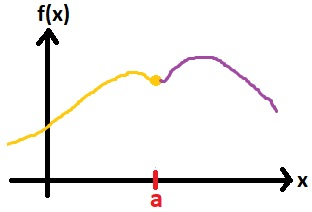
\includegraphics[scale=0.7]{img/continuity_plot.jpg}
\end{figure}

Hay una variedad de maneras en las que una función podría fracasar en ser continuas en el punto $x = a$. Una de ellas, es que \textbf{exita el límite de $f(x)$ cuando $x \to a$, pero no $f(a)$}. Es decir:

\begin{figure}[hbt!]
\centering
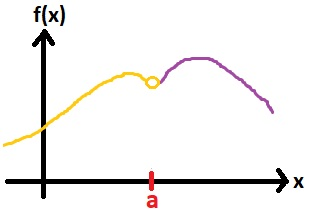
\includegraphics[scale=0.7]{img/continuity_plot_2.jpg}
\end{figure}

Como vemos, ahora el circulo en donde se une $f(x)$ cuando $x \to a^{-}$ y $x \to a^{+}$, está vacío, indicando que $f(a)$ no existe. Por consiguiente, $f(x)$ ya no es una función continua. A este caso se le denomina como \textbf{\underline{discontinuidad removible}}.

Otra forma en que no haya continuidad (o haya discontinuidad) en $f(x)$, es que \textbf{$f(a)$ y $\lim_{x \to a}f(x)$ existan, pero no sean iguales}. Es decir:
\[\lim_{x \to a}f(x) \neq f(a)\]
Gráficamente se vería de la siguiente manera:
\newpage
\begin{figure}[hbt!]
\centering
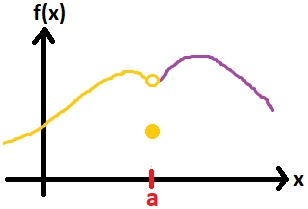
\includegraphics[scale=0.7]{img/continuity_plot_3.jpg}
\end{figure}

Finalmente, hay casos en donde \textbf{existe $f(a)$, pero no el $\lim_{x \to a} f(x)$}. Sabemos que hay distintas maneras en que el límite general no exista (ver pág. 11-12). Acá nos concentraremos en la instancia cuando \underline{existen los límites} de la izquierda y de la derecha de $f(x)$, \underline{pero no son iguales}. En ese momento el $\lim_{x \to a} f(x)$ no existe y, por consiguiente, $f(x)$ es discontinua en $x = a$. De manera que, en su gráfica, vamos a ver un \textbf{\underline{salto} en $x = a$}, similar al de a continuación:

\begin{figure}[hbt!]
\centering
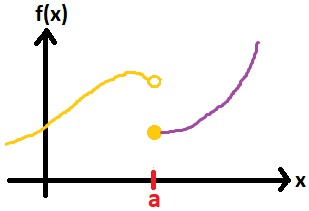
\includegraphics[scale=0.7]{img/continuity_plot_4.jpg}
\end{figure}

Ahora, como vemos en la figura de arriba, el límite de la izquierda de $f(x)$ (curva naranja) no es igual a $f(a)$, pero el límite de la derecha de $f(x)$ (curva morada) \textbf{sí es igual a $f(a)$}. Es decir:
\[\lim_{x \to a^{+}} f(x) = f(a)\]
En este caso, decimos que \textbf{$f(x)$ es \underline{continua a la derecha} en $x = a$}. Del mismo modo, cuando:
\[\lim_{x \to a^{-}} f(x) = f(a)\]
Señalamos que \textbf{$f(x)$ es \underline{continua a la izquierda} en $x = a$}.

No obstante y como ya se ha señalado, para que $f(x)$ sea continua en $x = a$:
\begin{enumerate}
\item Debe existir el $\lim_{x \to a} f(x)$ (límite general).
\item Debe existir $f(a)$.
\item $\lim_{x \to a} f(x) = f(a)$
\end{enumerate}

En ese sentido, cuando $f(x)$ es continua a la izquierda o a la derecha en $x = a$, aún así está siendo discontinua en general.

Por lo tanto, gráficamente, cuando $f(x)$ es discontinua en $x = a$, vamos a ver un círculo vacío si el límite existe, pero no $f(a)$; o un salto si $f(a)$ existe, pero no el límite. Y, en caso de ser continua, veremos que el límite se une en $x = a$ y aquel círculo está cerrado.


\subsection{Continuidad General.}

Hasta ahora hemos visto que una función puede ser continua en un punto. Del mismo modo, también revisamos que en ciertos puntos puede ser continua y en otros, discontinua. Pero \textbf{¿qué ocurre cuando una función es continua en todos los puntos?}

Si una función es continua en todos los puntos, entonces decimos que es \textbf{continua en todos los $\mathbb{R}$}. De hecho, cuando decimos que una función es continua, sin decir que lo es en un punto, nos estamos refiriendo a esta continuidad o \textbf{continuidad general}.

Cuando decimos que una función es continua, quiere decir que \textbf{en ninguna parte de la función hay discontinuidad}, es decir, no hay círculos vacíos o saltos, solo es una línea (curva o recta) sin interrupciones\footnote{Es como si dibujaramos una línea sin levantar el lápiz.}.

Las funciones continuas son muy útiles para calcular sus límites, porque siempre serán iguales. Es decir, para realizar dicho cálculo solo debemos buscar cuál es el valor de aquella función en algún punto del eje $x$.

Veamos como ejemplo la siguiente función constante: $f(x) = 3$

\begin{figure}[hbt!]
\centering
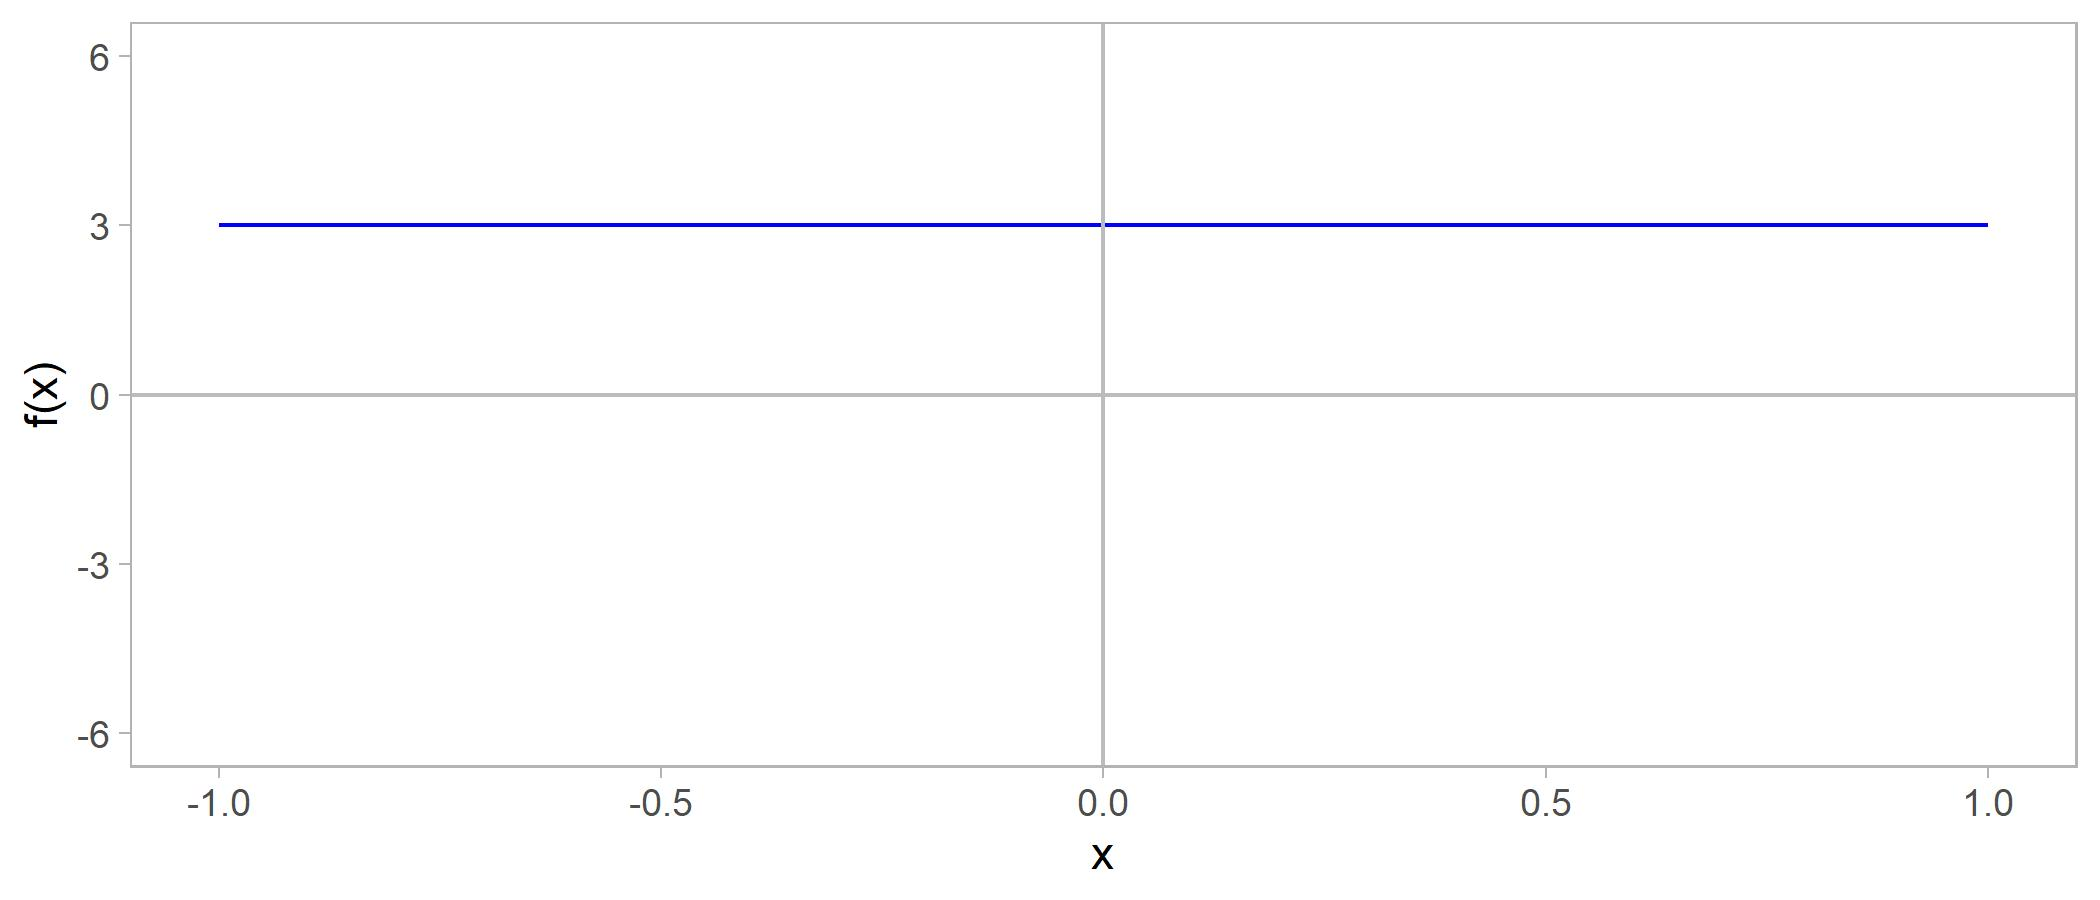
\includegraphics[scale=0.7]{img/continuity_f.jpg}
\end{figure}

Como vemos, en $f(x)$ no hay alguna discontinuidad para todos los valores $x$, de manera que es continua. De hecho, todas las funciones constantes, son continuas, por el mismo motivo.

Revisemos otra básica función que es continua en general: la función afín, que denotaremos como $g(x) = x$.

\begin{figure}[hbt!]
\centering
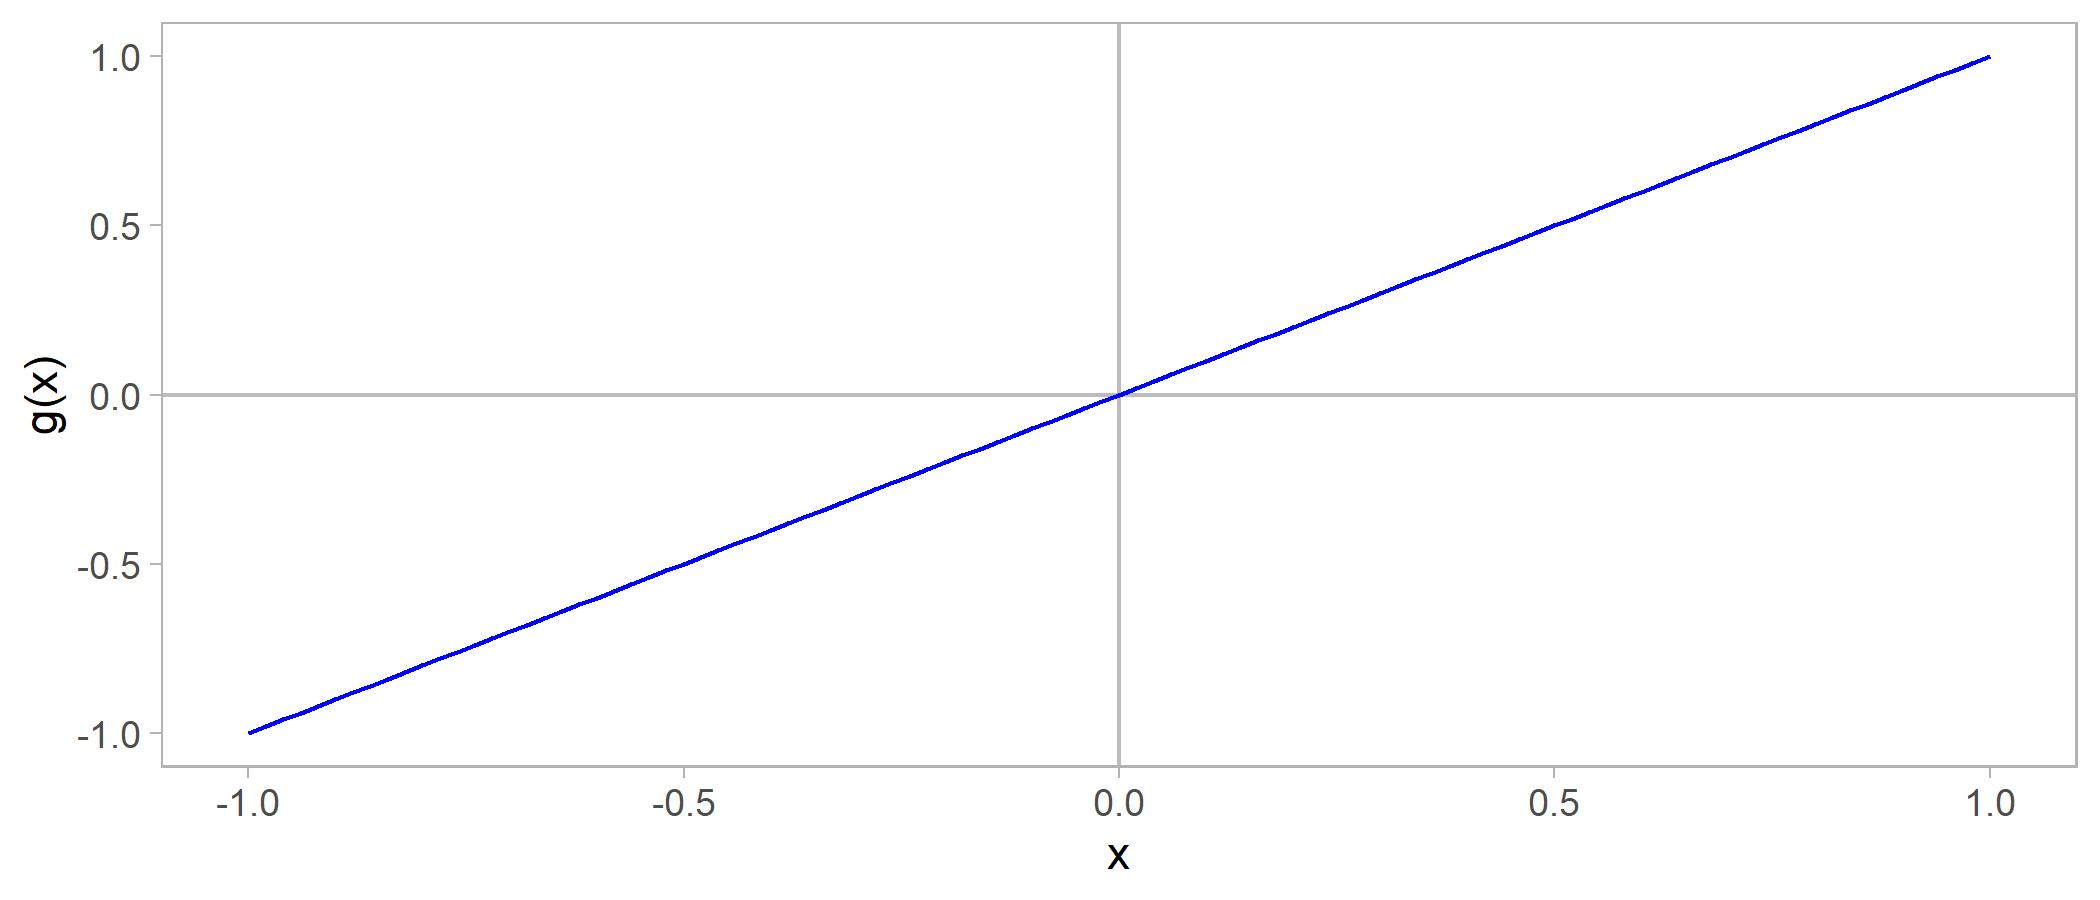
\includegraphics[scale=0.7]{img/continuity_g.jpg}
\end{figure}

\newpage

O, también, la función valor absoluto $h(x) = |x|$, que como podemos ver en el siguiente gráfico, tampoco tiene hoyos o círculos vacíos, saltos, etc. Ninguna discontinuidad.

\begin{figure}[hbt!]
\centering
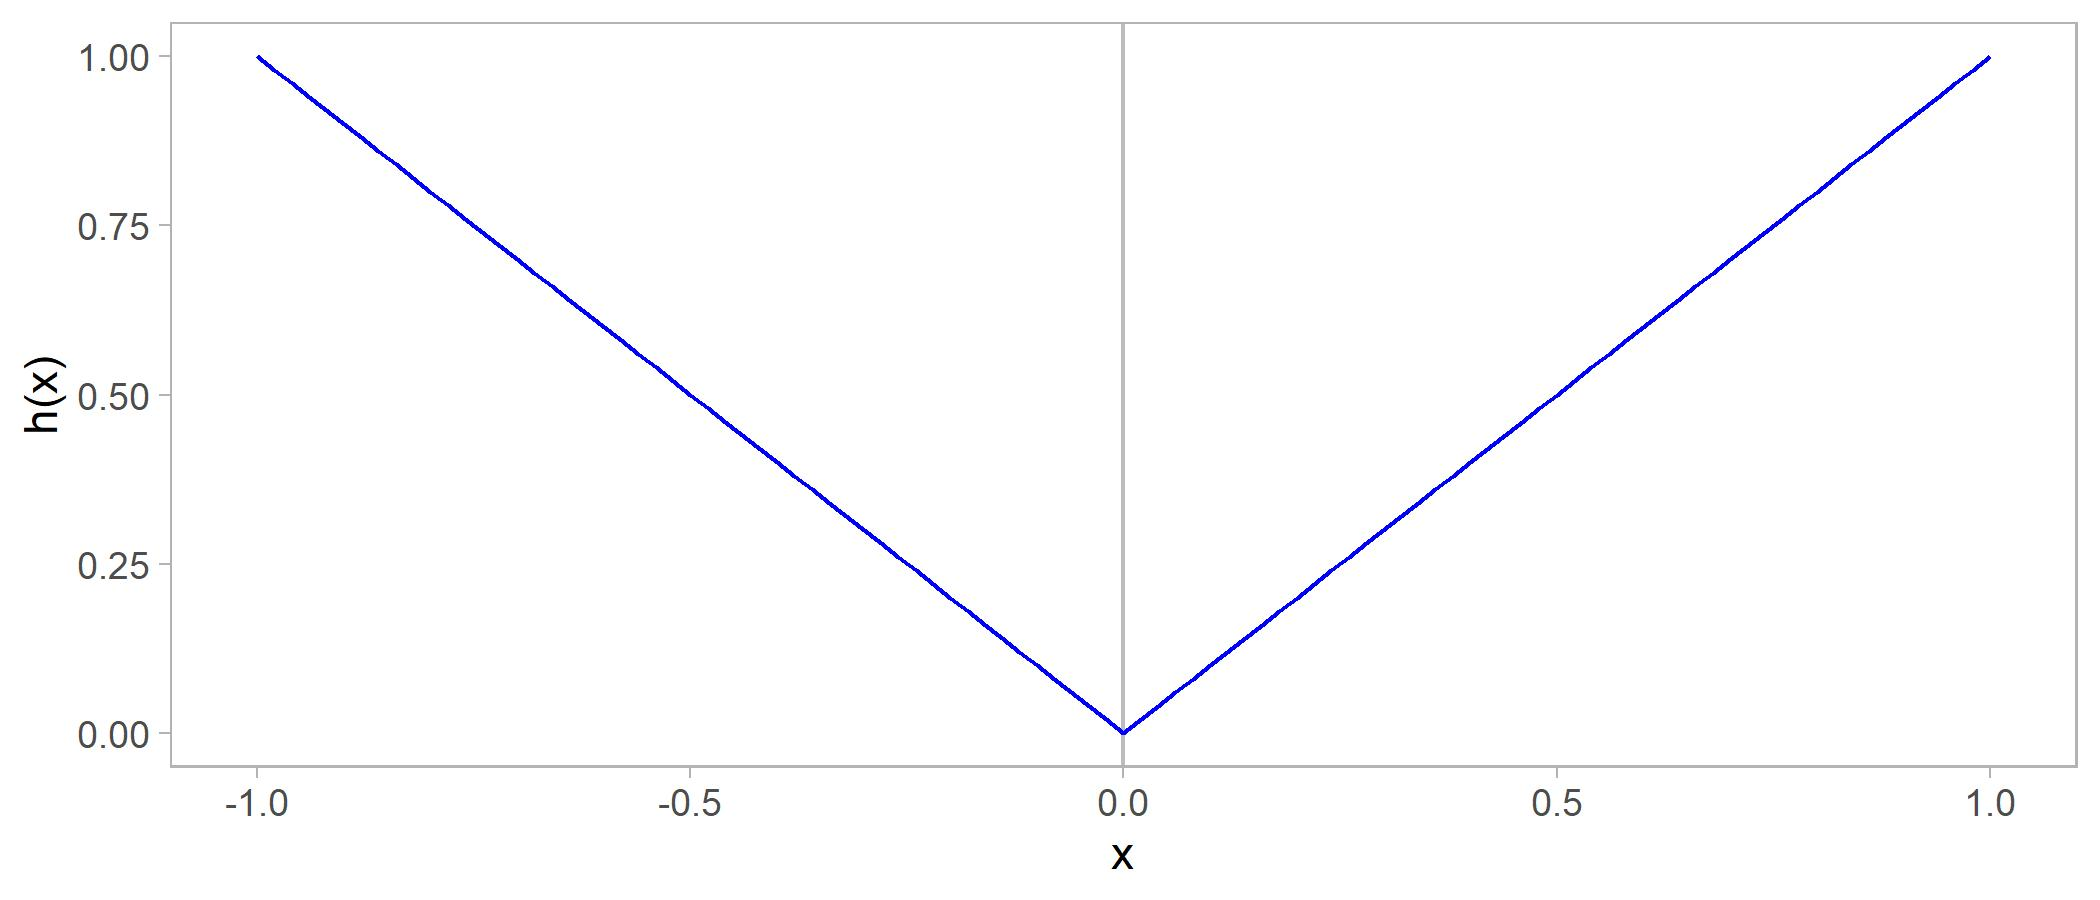
\includegraphics[scale=0.7]{img/continuity_h.jpg}
\end{figure}

Otras funciones que también son continuas, son la función $sen(x)$ y la función $cos(x)$.

\begin{figure}[hbt!]
\centering
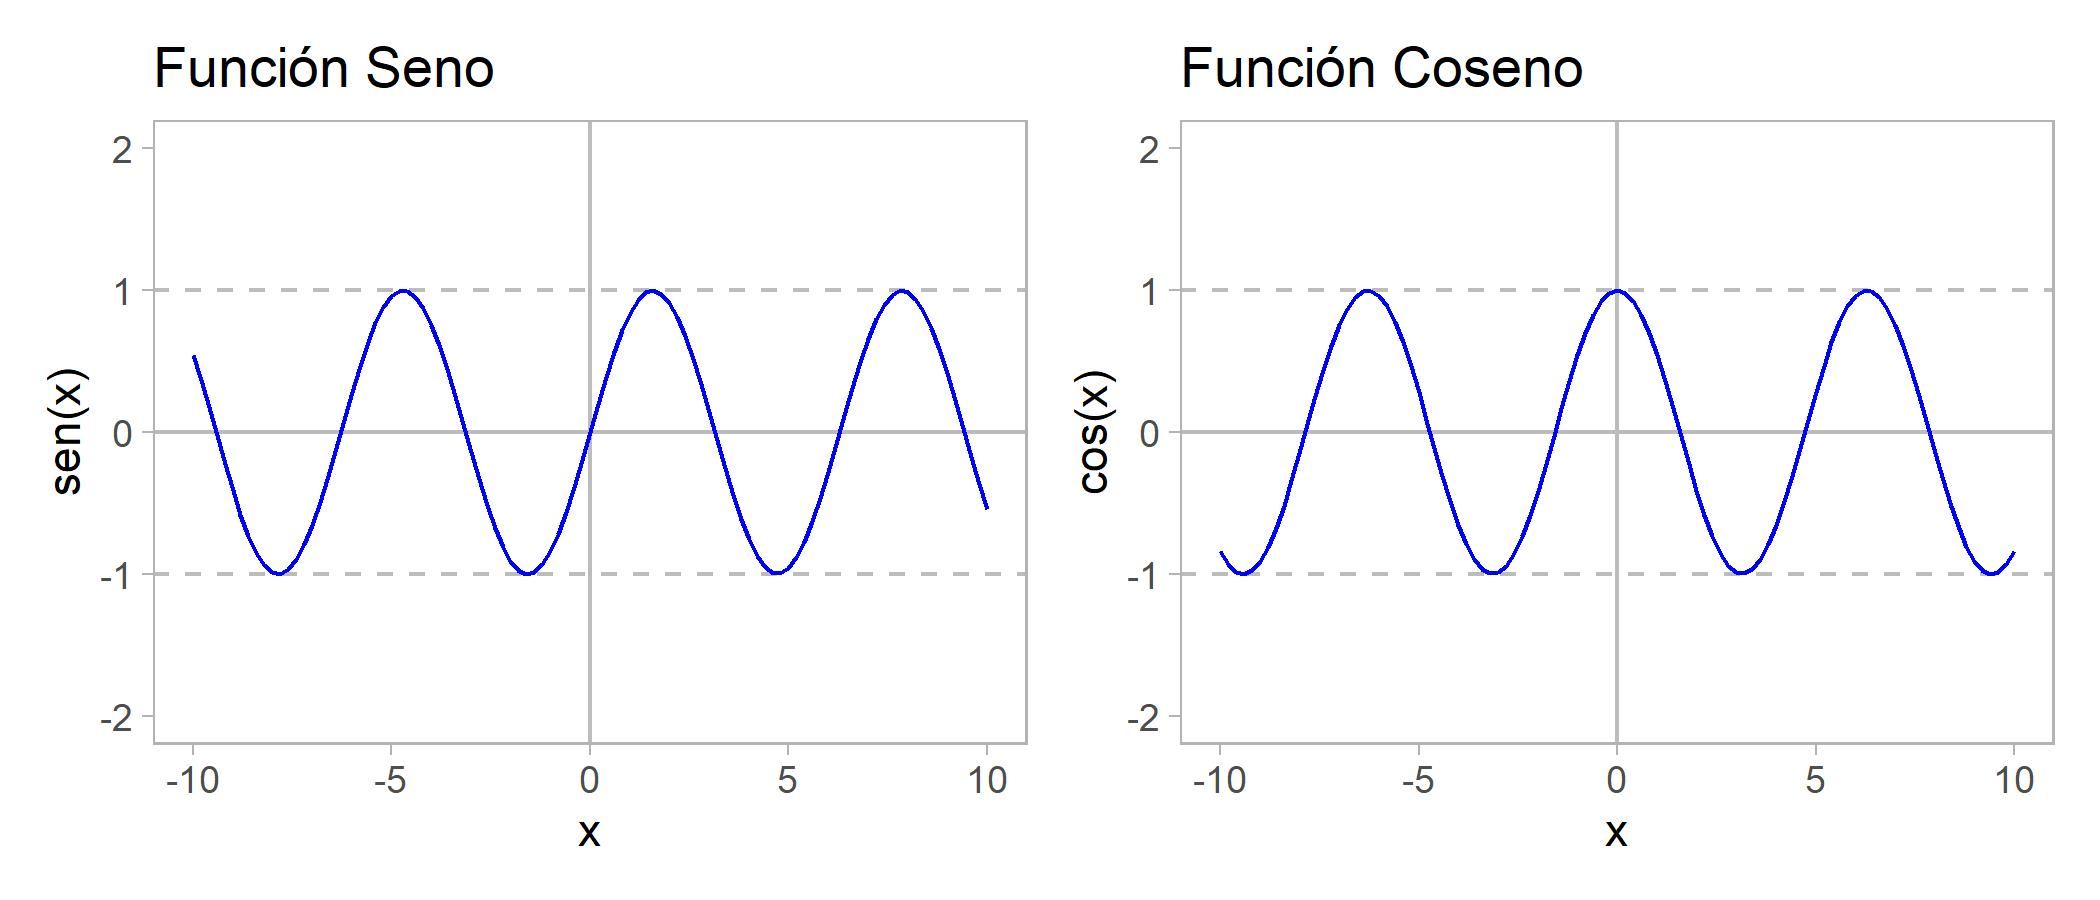
\includegraphics[scale=0.7]{img/sen_cos_continuity.jpg}
\end{figure}

Sin embargo, un ejemplo de discontinuidad, es la función $tan(x)$. Recordemos que se calcula como:
\[tan(x) = \frac{sen(x)}{cos(x)}\]
Esto quiere decir que la $tan(x)$ no está definida cuando $cos(x) = 0$, de manera que es continua en todos los puntos, menos cuando $cos(x) = 0$.

Por lo tanto, muchas de nuestras funciones básicas son continuas, pero no todas, por lo que debemos ser cuidadosos a la hora de determinar si lo son o si son discontinuas.


\subsection{Leyes de los Límtes y Continuidad.}

En esta ocasión, veremos qué es lo que nos dicen las leyes de los límites con respecto a la continuidad de una función.

Digamos que tenemos dos funciones: $f(x)$ y $g(x)$ y ambas son continuas en el punto $x = a$. Esto implica, por definición, que sus límites calzan con el valor de sus funciones en el punto $a$.
\[\lim_{x \to a} f(x) = f(a)\]
\[\lim_{x \to a} g(x) = g(a)\]
Y supongamos que tenemos la siguiente combinación de funciones:
\[h(x) = f(x) \times g(x)\]
\textbf{¿Qué podemos decir de la continuidad de $h(x)$?} Como vimos antes (pág. 15), el límite de un producto es el producto de dos límites.
\[\lim_{x \to a} h(x) = \lim_{x \to a}[f(x) \times g(x)]\]
\[\lim_{x \to a} h(x) = \lim_{x \to a} f(x) \times \lim_{x \to a} g(x)\]
Y acabamos de ver que $\lim_{x \to a} f(x) = f(a)$ y $\lim_{x \to a} g(x) = g(a)$. Entonces:
\[\lim_{x \to a} h(x) = f(a) \times g(a)\]
Es decir, cuando $x \to a$, $h(x)$ se está acercando al valor $f(a) \times g(a)$. Lo que significa que:
\[h(a) = f(a) \times g(a)\]
Por consiguiente:
\[\lim_{x \to a} h(x) = h(a)\]
Es decir, \textbf{$h(x)$ es una función continua}.

Lo que acabamos de demostrar es que \textbf{si $f(x)$ y $g(x)$ son \underline{continuas en un punto}, entonces \underline{su producto} será \underline{continua en ese punto}}.

Por consiguiente, si $f(x)$ y $g(x)$ \textbf{son continuas en general, dicho producto también será continua en general}.

Este último punto \textbf{también ocurre para las leyes de los límites de la suma y la resta}.

A partir de estos principios podemos deducir que muchas funciones son continuas. Por ejemplo, veamos si la composición de $h(x)$ entre una función constante $f(x) = 5$ y una afín $g(x) = x$, es una función continua.

Anteriormente vimos (pág. 20) que las funciones constantes y afines, son continuas en general (i.e., para todos los $\mathbb{R}$). Por lo tanto, si aplicamos la ley del límite para el producto, la suma o resta de los límites en $h(x)$, esta función será continua en general. 

Veamos en la ley del límite para el producto en un punto $x = a$:
\[\lim_{x \to a} h(x) = \lim_{x \to a} f(x) \times \lim_{x \to a} g(x)\]
\[\lim_{x \to a} h(x) = f(x) \times g(x)\]
\[\lim_{x \to a} h(x) = 5 \times x\]
\[\lim_{x \to a} h(x) = 5x\]
Acabamos de decir que las funciones constantes y afines son continuas en general, entonces $h(x)$ no solo será continua en $x=a$, sino que en todos los valores de $x$ que pertenecen a $\mathbb{R}$ (i.e., es continua en general). Por lo tanto:
\[h(x) = 5x\]
En ese sentido, si multiplicamos nuestra nueva $h(x)$ por otra función afín $j(x) = x$, obtendremos otra función continua general:
\[\lim_{x \to a} k(x) = h(x) \times j(x)\]
\[\lim_{x \to a} k(x) = 5x \times x\]
\[\lim_{x \to a} k(x) = 5x^{2}\]
Lo mismo si le sumamos otra función afín $p(x) = x$ a esta última:
\[\lim_{x \to a} n(x) = k(x) + p(x)\]
\[\lim_{x \to a} n(x) = 5x^{2} + x\]
Básicamente, \textbf{cualquier polinomio es una función continua en general}.

Ahora bien, no nos olvidemos que tenemos \textbf{la ley del límite para el cuociente} de funciones. En ésta, también una función puede ser continua en general, \textbf{salvo cuando el denominador es igual a cero}. En este caso se indefinirá, por lo que será discontinua en ese punto. Es decir, una función compuesta por una división entre funciones, será continua donde está definida.

Volvamos a ver el ejemplo de la $tan(x)$. Como sabemos, es el cuociente entre el $sen(x)$ y el $cos(x)$, ambas funciones continuas en general. Por lo tanto, $tan(x)$ va a ser continua en general en todos los puntos de la recta real, salvo cuando $cos(x) = 0$.

Por otra parte, la siguiente función $f(x)$, sí es continua en general.
\[f(x) = \frac{1}{x^{2}+1}\]
Comprobémoslo calculando su límite, cuando $x \to a$.
\[\lim_{x \to a} f(x) = \lim_{x \to a} \left[\frac{1}{x^{2}+1}\right]\]
\[\lim_{x \to a} f(x) = \frac{\lim_{x \to a} 1}{\lim_{x \to a} [x^{2} + 1]}\]
Ya sabemos que las funciones constantes (númerador), son continuas en general. Ahora bien, no todas las polinómicas son continuas, sin embargo, la que está en el denominador ($x^{2} + 1$) nunca será igual a cero y será continua en todos los valores del conjunto de los $\mathbb{R}$. Por lo tanto, la función:
\[f(x) = \frac{1}{x^{2}+1}\]
Será continua en general.

Ahora veamos el caso de una \textbf{composición de funciones}. 

\underline{Ejemplo}: Si $f$ y $g$ son funciones continuas en general, ¿qué podemos decir sobre $h(x) = f(g(x))$?

\underline{Respuesta}: Sabemos que $g(x)$ es continua en general, por lo que si, por ejemplo, $x \to a$, entonces $g(x) \to g(a)$.

Por otra parte, también tenemos conocimiento de que $f$ es continua en general en $g(x)$, de manera que si $x \to a$, $f(g(x)) \to f(g(a))$. En otras palabras, cuando $x \to a$, $h(x) \to h(a)$. Por lo tanto, podemos decir que $h(x)$ es continua en el punto $x = a$.

Entonces, es posible señalar que si $f$ y $g$ son funciones continuas en general, entonces \textbf{la composición $f \, o \, g$, es continua en todos lados}.

Veamos otra composición de dos funciones: $sen(x^{2} + 1)$. Las dos funciones, son las siguientes:
\begin{enumerate}
\item $(x^{2} + 1)$
\item $sen(x)$
\end{enumerate}

Como ya hemos visto, las funciones polinomias son continuas en general y la función seno, también. Por lo tanto, podemos señalar que $sen(x^{2} + 1)$, es una función continua general.

Para terminar, resumamos toda la información que hemos revisado en este apartado.

Sean las funciones $f$ y $g$, continuas en general:
\begin{itemize}
\item $f \times g \rightarrow$ Continua en general.
\item $f + g \rightarrow$ Continua en general.
\item $f - g \rightarrow$ Continua en general.
\item $f/g \rightarrow$ Continua en general donde esté definida (i.e., donde $g \neq 0$).
\item $f \, o \, g \rightarrow$ Continua en general.
\end{itemize}

También podemos hacer un catálogo con aquellas funciones que son continuas en todos los reales y en solo algunos valores:

\underline{Continuas en los Reales ($\mathbb{R}$)}.

\begin{itemize}
\item Todos los polinomios.
\item $\sqrt[3]{x}$
\item $|x|$
\item $cos(x)$ y $sen(x)$
\item Funciones exponenciales $a^{x}$ con $a > 0$
\end{itemize}

\underline{Continuas (a la derecha) en valores específicos de $x$}.

\begin{itemize}
\item $\sqrt{x}$ para todo $x \geq 0$
\item $tan(x)$ en todos los $x$ en donde esté definida (i.e., $cos(x)\neq 0$).
\item Funciones logarítmicas $\log_{a}x$, donde la base $a >0$ para todo $x > 0$.
\end{itemize}


\subsection{Introducción al Teorema del Valor Intermedio.}

Digamos que, en un gráfico, tenemos dos puntos: $(a, \, f(a))$ y $(b, \, f(b))$; y también una línea horizontal $y = M$.

\begin{figure}[hbt!]
\centering
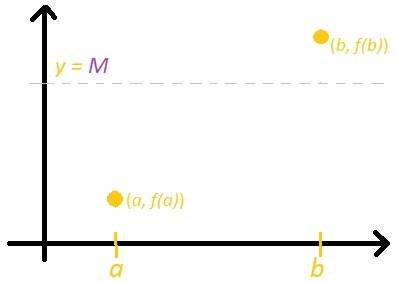
\includegraphics[scale=0.7]{img/intermed_value_teo.jpg}
\end{figure}

La pregunta que vamos a contestar a continuación es si, al viajar la gráfica de $f$ desde el punto $(a, \, f(a))$ hasta $(b, \, f(b))$, \textbf{¿va a intersectar a la recta $y = M$?}

La respuesta será \textbf{sí, siempre y cuando $f$ sea \underline{continua}.} En otras palabras, mientras se cumpla esta condición, \textbf{la gráfica de la función $f$ va a intersectar a la recta $y = M$ en, al menos, un punto de ella} (i.e., puede cortar en 1 o más puntos de $y = M$).

A esto se le denomina como el \textbf{Teorema del Valor Intermedio} y señala lo siguiente:
\begin{quotation}
Si una función $f$ es continua y un valor $M$ está entre $f(a)$ y $f(b)$ (i.e., un valor intermedio), entonces hay, al menos, un punto $c$ entre $a$ y $b$, tal que $f(c) = M$.
\end{quotation}

\begin{figure}[hbt!]
\centering
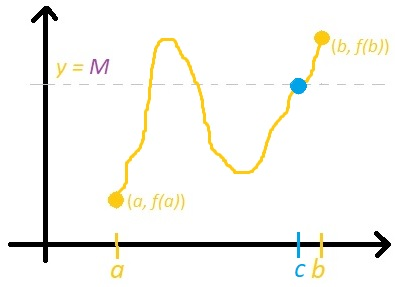
\includegraphics[scale=0.7]{img/intermed_value_teo_2.jpg}
\end{figure}

Por lo tanto, para que haya al menos un punto $c$ entre los puntos $a$ y $b$, tal que $f(c) = M$, deben cumplirse los siguientes requisitos:
\begin{itemize}
\item La función $f$ debe ser continua.
\item El valor $M$ debe estar entre $f(a)$ y $f(b)$.
\end{itemize}

Ahora bien, algo importante a señalar es que \textbf{sí o sí la función $f$ debe ser continua entre los puntos $(a, \, f(a))$ y $(b, \, f(b))$}. Afuera de ellos pueden haber discontinuidades. En otras palabras, la función $f$ debe ser:
\begin{itemize}
\item Continua general en el conjunto $[a, \, b]$.
\item Continua hacia la derecha en el punto $x = a$.
\item Continua hacia la izquierda en el punto $x = b$.
\end{itemize}

Por lo tanto, si se cumplen las anteriores condiciones, más que $M$ esté entre $f(a)$ y $f(b)$, entonces la función $f$ va a ser igual a $M$ en al menos un punto de su recta (i.e., $f(c) = M$).

\newpage


\subsection{Aplicando el Teorema del Valor Intermedio.}

Comencemos con el siguiente polinomio: $x^{4} - x - 1$, y digamos que queremos saber si tiene alguna raíz. ¿Alguna vez es igual a cero? Es decir:
\[x^{4} - x - 1 = 0 ?\]
Podríamos partir factorizando este polinomio, pero nos tomará un tiempo de más, así que veamos otro camino.

Como mencionamos antes (pág. 26), todos los polinomios son continuos en general. Por lo tanto, si decimos que aquel polinomio es una función, entonces podemos aplicar el teorema del valor intermedio, porque lo que queremos saber es si hay algún punto ``$c$'' en $x$ tal que $f(c) = 0$.

Ya sabemos que $x^{4} - x - 1$ es continua en general, así que solo debemos buscar $f(a)$ y $f(b)$; y ver si $f(c) = 0$ está entremedio de las dos anteriores funciones.

Sea $f(x) = x^{4} - x - 1$, usaremos los valores $x = \{1, \, 3\}$ para construir la siguiente tabla:

\begin{center}
\begin{tabular}{c | c}

$x$ & $f(x)$\\
\hline
1 & -1\\
3 & 77\\

\end{tabular}
\end{center}

Como vemos, el valor $f(x) = 0$ (o $y = 0$) está entre los valores $f(1) = -1$ y $f(3) = 77$. Por lo tanto, podemos señalar que hay, al menos, un lugar en el espacio en donde $f(x)$ intersecta al eje $x$ en $y = 0$.
\newpage
\begin{figure}[hbt!]
\centering
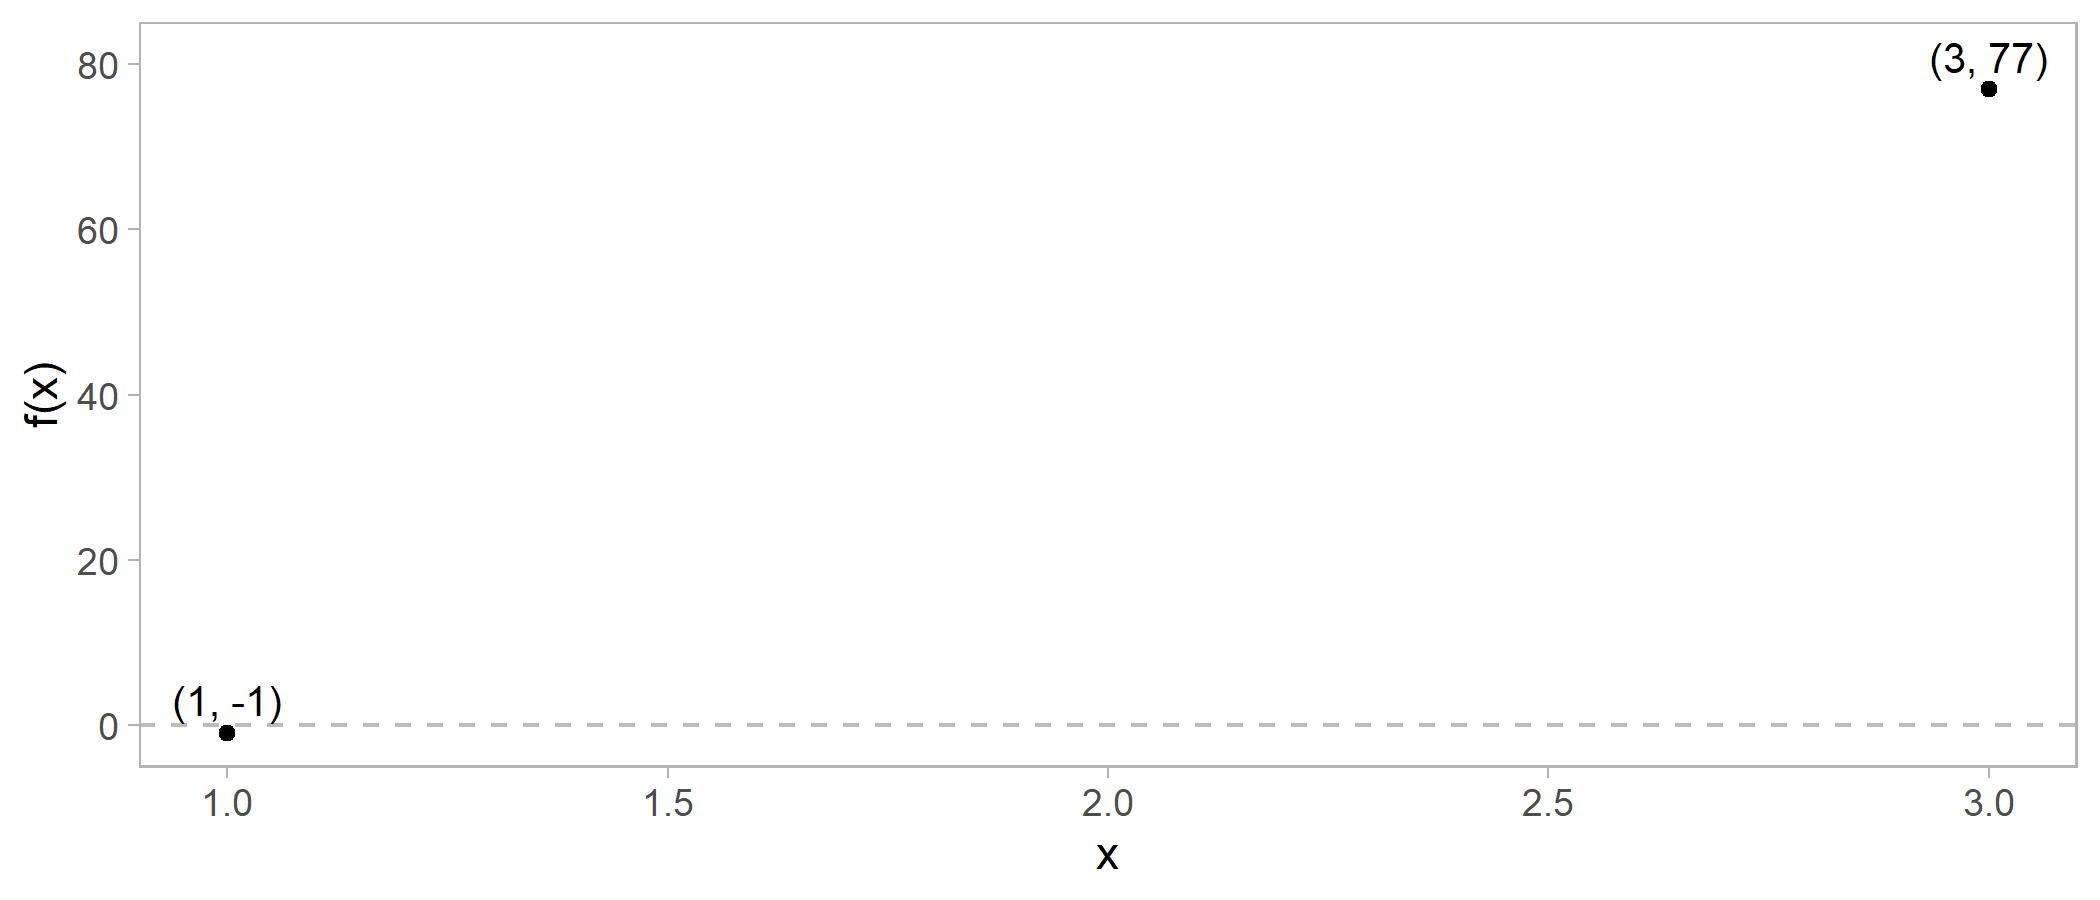
\includegraphics[scale=0.7]{img/interm_value_plot.jpg}
\end{figure}

El Teorema del Valor Intermedio no nos dice en qué punto del eje $x$ la función $f(x)$ intersectará a $y = 0$. Simplemente nos indica que va a intersectar alguna vez, una o más veces la recta $y = 0$.


\subsection{Límites y División.}

Previamente, hablamos sobre las ley del cuociente para los límites (pág. 15).
\[\lim_{x \to a} \left[\frac{f(x)}{g(x)}\right]\]
En particular, señalamos que si el $\lim_{x \to a} f(x) = L$, el $\lim_{x \to a} g(x) = M$ y si $M \neq 0$, entonces:
\[\lim_{x \to a} \left[\frac{f(x)}{g(x)}\right] = \frac{L}{M}\]
La pregunta que vamos a abordar a continuación, es: \textbf{¿qué ocurre si \underline{$M = 0$?}} O, en otras palabras, ¿qué ocurre con la ley del cuociente si el denominador $\lim_{x \to a} g(x) = 0$? Esto va a depender de lo que esté ocurriendo en el numerador.

\underline{Caso 1}: Que $L \neq 0$ cuando $M = 0$.

Si $M = 0$, pero $L \neq 0$, cuando vemos la división entre $f(x)$ y $g(x)$ mientras $x \to a$, \textbf{el numerador $L$ nunca se va a acercar a cero}. En otras palabras, va aumentando cada vez más mientras $x \to a$. Por otra parte, en ese mismo caso ($x \to a$), el denominador $g(x)$ sí se va haciendo muy pequeño, de manera que $M \to 0$.

En este caso, lo anterior implica que, mientras $x \to a$, vamos a estar calculando un cuociente entre un número cada vez más grande (numerador) con uno cada vez más pequeño (denominador), el cual va a terminar siendo un número enorme y tanto en sentido positivo como negativo. Es decir:

Mientras $x \to a$
\[\frac{f(x)}{g(x)} = \frac{N^{o} \, grande}{N^{o} \, chico} = \pm N^{o} \, Enorme\]
Y, cuando el denominador $N^{o} \, chico = 0$, entonces el cuociente que acabamos de ver, se indefine.

Más allá de lo anterior, una cosa que es segura es que mientras $x$ se acerque a un número (i.e., mientras $x \to a$), el cuociente $f(x)/g(x)$ \textbf{nunca será un número fijo}.

Por lo tanto, como conclusión a este caso podemos señalar que si $M = 0$ y $L \neq 0$, entonces:
\[\lim_{x \to a} \left[\frac{f(x)}{g(x)}\right] = No \, Existe\]

\underline{Caso 2}: Que $L = 0$ cuando $M = 0$.

De este último caso, surge otro: Si $L = 0$ cuando $M = 0$, en otras palabras, que tanto el numerador como el denominador, sean iguales a cero. Podría tentarnos a decir automáticamente que el límite no existe, pero no siempre es el caso. Veamos el siguiente ejemplo:
\[\lim_{x \to 0} \frac{2x}{x}\]
Como vemos, ambas funciones ($2x$ y $x$) son continuas, de manera que si $x \to 0$, entonces $2x \to 0$ y $x \to 0$. Pero no queremos que ambas sean iguales a cero. En otras palabras, no queremos decir que:
\[\lim_{x \to 0} \frac{2x}{x} = \frac{0}{0}\]
Porque no está definida.

No obstante, podemos calcular el cuociente entre $2x$ y $x$:
\[\frac{2x}{x} = 2\]
Por lo tanto, el límite nos quedaría como:
\[\lim_{x \to 0} \frac{2x}{x} = \lim_{x \to 0} 2 = 2\]
En realidad, el límite va a ser igual a 2, \textbf{pero siempre y cuando el denominador $x \neq 0$}. No obstante, cuando calculamos el límite mientras $x \to 0$, lo que ocurra cuando $x = 0$ no nos tiene que importar, porque mientras eso suceda, $2x$ nunca va a ser igual a cero y $x$ tampoco. Por lo tanto, el límite va a ser igual a 2 en todos lados.

Quizá podríamos pensar que este último caso (que exista el límite de un cuociente, cuando el numerador y el denominador son iguales a cero) es una excepción, sin embargo, hay muchos casos en Cálculo en donde ésto ocurre.

Para terminar, resumamos los casos que hemos visto, incluyendo el que vimos anteriormente en las Leyes de los Límites (pág. 15).

Sea $f(x) = L$ y $g(x) = M$.

\underline{Caso 0}:

Si $M \neq 0$, entonces:
\[\lim_{x \to a} \frac{f(x)}{g(x)} = \frac{L}{M}\]
\underline{Caso 1}:
Si $M = 0$, pero $L \neq 0$, entonces:
\[\lim_{x \to a} \frac{f(x)}{g(x)} = No \, Existe\]
\underline{Caso 2}:
Si $M = 0$ y $L = 0$, entonces:
\[\lim_{x \to a} \frac{f(x)}{g(x)} = No, \, necesariamente, \, no \, existe\]


\subsection{Pequeño Dividido por Pequeño.}

En esta ocasión vamos a profundizar en la ley del cuociente para el límite, principalmente cuando los límites del numerador y el del denominador, son iguales a cero, pero sin que éste sea igual a $0/0$. Recordemos que cuando $x \to a$, entonces $f(x)/g(x) \to 0$, pero no es igual a cero (i.e., $f(x)/g(x) \neq 0$ cuando $x \to a$).

Por lo tanto, cuando $x \to a$:
\[\frac{f(x)}{g(x)} = \frac{n^{o} \, chico}{n^{o} \, chico}\]
Algo interesante de ésto, es que el tener conocimento de que el numerador o el denominador es un número pequeño, no nos dice nada sobre qué tan enorme (\textit{huge}) es el cuociente entre ellos. Lo que sí necesitamos saber es \textbf{qué tan pequeño es el numerador o el denominador en relación al otro}.

Por ejemplo, el numerador puede ser un número pequeño (e.g., $0.01$), pero el denominador puede serlo aún más ($0.00001$).
\[\frac{0.01}{0.00001} = 1000\]
O puede ocurrir al revés:
\[\frac{0.00001}{0.01} = 0.001\]
Veamos el caso de la sección anterior:
\[\lim_{x \to 0}\left[\frac{2x}{x}\right]\]
Como podemos apreciar, el denominador es la mitad del numerador, por lo que el cuociente entre ambas será igual a 2:
\[\lim_{x \to 0}\left[\frac{2x}{x}\right] = 2\]
Lo que podemos concluir de ésto es que si tanto el numerador como el denominador van a tender a ser iguales a cero, entonces el cuociente entre ambos, puede ser cualquier resultado. Podría ser un número enorme o uno pequeño o estar entremedio de ambos. Esto último no quiere decir que nos rendimos y, simplemente, no sabemos cuál es el resultado exacto de aquel cuociente. Más bien, significa que \textbf{tenemos que trabajar mucho más para determinar cuál es el límite en cada caso en donde el numerador y el denominador puedan acercarse a ser iguales a cero}.



\subsection{Aplicando la Ley del Límite para el Cuociente.}

Ahora apliquemos los tres casos que hemos visto sobre la ley del límite para el cuociente. Recordemos cuáles son:

1. \underline{Caso 1}:

Si el $\lim_{x \to a}f(x) = L$ y $\lim_{x \to a} g(x) \neq 0$, entonces:
\[\lim_{x \to a} \left[\frac{f(x)}{g(x)}\right] = \frac{L}{M}\]
2. \underline{Caso 2}:

Si el $\lim_{x \to a}f(x) = 0$ y $\lim_{x \to a} g(x) \neq 0$, entonces:
\[\lim_{x \to a} \left[\frac{f(x)}{g(x)}\right] = No \, Existe\]

\newpage

3. \underline{Caso 3}:

Si el $\lim_{x \to a}f(x) = 0$ y $\lim_{x \to a} g(x) = 0$, entonces debemos trabajar más para determinar:
\[\lim_{x \to a} \left[\frac{f(x)}{g(x)}\right]\]

Veamos el siguiente ejemplo:

\underline{Ejemplo 1}:
\[\lim_{x \to 0} \left[\frac{x^{2} + 2x - 3}{x^{2} - 3x + 2}\right]\]
\underline{Respuesta 1}: Observemos primero el denominador. Como podemos apreciar, es un polinomio y ya sabemos que todos los límites de las funciones que son polinomios, son continuas en general\footnote{Recordemos que cuando una función es continua, entonces $\lim_{x \to a} f(x) = f(a)$.}. Por lo tanto:
\[\lim_{x \to 0}[x^{2} - 3x + 2] = 0^{2} - (3 \times 0) + 2\]
\[\lim_{x \to 0}[x^{2} - 3x + 2] = 2\]
Del mismo modo, también podemos ver que el numerador es un polinomio, por consiguiente:
\[\lim_{x \to 0}[x^{2} + 2x - 3] = 0^{2} - (2 \times 0) - 3\]
\[\lim_{x \to 0}[x^{2} + 2x - 3] = -3\]
Ahora revisemos cómo quedó el cuociente:
\[\frac{- 3}{2}\]
En otras palabras, está ocurriendo el ``\underline{Caso 1}'', por lo que el límite existe y va a ser el cuociente entre aquellos dos valores.
\[\lim_{x \to 0} \left[\frac{x^{2} + 2x - 3}{x^{2} - 3x + 2}\right] = \frac{- 3}{2}\]

\underline{Ejemplo 2}: Veamos ahora el mismo límite, pero con $x \to 1$.
\[\lim_{x \to 1} \left[\frac{x^{2} + 2x - 3}{x^{2} - 3x + 2}\right]\]
\underline{Respuesta 2}: De nuevo, tanto las funciones del numerador como del denominador, son continuas, por lo que podemos aplicar esta regla para conocer sus límites. Partamos con el numerador:
\[\lim_{x \to 1} [x^{2} + 2x - 3] = 1^{2} + (2 \times 1) - 3\]
\[\lim_{x \to 1} [x^{2} + 2x - 3] = 0\]
Calculemos el denominador:
\[\lim_{x \to 1} [x^{2} - 3x + 2] = 1^{2} - (3 \times 1) + 2\]
\[\lim_{x \to 1} [x^{2} - 3x + 2] = 0\]
Por lo tanto, ahora estamos tratando con el ``\underline{Caso 3}'', en donde tanto el numerador como el denominador, son iguales a cero. Cuando ocurre este caso y estamos \underline{trabajando con polinomios}, lo que debemos hacer es \textbf{\underline{factorizarlos}}. Es decir:
\[\lim_{x \to 1} \left[\frac{x^{2} + 2x - 3}{x^{2} - 3x + 2}\right] = \lim_{x \to 1} \left[\frac{(x + 3)(x - 1)}{(x - 2)(x - 1)}\right]\]
\[\lim_{x \to 1} \left[\frac{x^{2} + 2x - 3}{x^{2} - 3x + 2}\right] = \lim_{x \to 1} \left[\frac{x + 3}{x - 2}\right]\]
Luego de haber factorizado ambos polinomios, podemos calcular el límite de nuestra nueva división. Como podemos observar, tanto el numerador como el denominador, nuevamente son funciones continuas. Así que podemos usar el mismo método usado en las ocasiones anteriores con los polinomios.
\[\lim_{x \to 1} \left[\frac{x + 3}{x - 2}\right] = \frac{\lim_{x \to 1} x + 3}{\lim_{x \to 1} x - 2}\]
\[\lim_{x \to 1} \left[\frac{x + 3}{x - 2}\right] = \frac{1 + 3}{1 - 2}\]
\[\lim_{x \to 1} \left[\frac{x + 3}{x - 2}\right] = \frac{4}{-1}\]
Por consiguiente, ahora nos encontramos con el ``\underline{Caso 1}'', de manera que el límite, en realidad, sí existe y va a ser el cuociente entre $4$ y $-1$, es decir:
\[\lim_{x \to 1} \left[\frac{x + 3}{x - 2}\right] = -4\]

\underline{Ejemplo 3}: Calculemos el siguiente límite:
\[\lim_{x \to -1} \left[\frac{x + 1}{x + \frac{1}{x} + 2}\right]\]
\underline{Respuesta 3}: Veamos primero qué está ocurriendo con el denominador mientras $x \to -1$
\[\lim_{x \to -1} \left[x + \frac{1}{x} + 2\right] = -1 + \frac{1}{-1} + 2\]
\[\lim_{x \to -1} \left[x + \frac{1}{x} + 2\right] = 0\]
Ahora observemos el numerador:
\[\lim_{x \to -1} [x + 1] = -1 + 1\]
\[\lim_{x \to -1} [x + 1] = 0\]
Otra vez nos hemos encontrado con el ``\underline{Caso 3}''.
\[\lim_{x \to -1} \left[\frac{x + 1}{x + \frac{1}{x} + 2}\right] = \frac{0}{0}\]
A diferencia del caso anterior, no podemos factorizar ambas expresiones algebraicas como lo hicimos antes, debido a la fracción que hay en el denominador. Lo que sí podemos hacer, primero, es multiplicar por $x$ tanto el numerador como el denominador, para sacarnos de encima de aquella fracción de esta última parte.
\[\lim_{x \to -1} \left[\frac{x + 1}{x + \frac{1}{x} + 2}\right] = \frac{x(x + 1)}{x(x + \frac{1}{x} + 2)}\]
\[\lim_{x \to -1} \left[\frac{x + 1}{x + \frac{1}{x} + 2}\right] = \frac{x^{2} + x}{x^{2} + 1 + 2x}\]
Ahora podemos calcular el límite de esta nueva fracción, mientras $x \to -1$.
\[\lim_{x \to -1} \left[\frac{x^{2} + x}{x^{2} + 1 + 2x}\right] = \frac{\lim_{x \to -1} [x^{2} + x]}{\lim_{x \to -1} [x^{2} + 1 + 2x]}\]
\[\lim_{x \to -1} \left[\frac{x^{2} + x}{x^{2} + 1 + 2x}\right] = \frac{-1^{2} + (-1)}{-1^{2} + 1 + (2 \times -1)}\]
\[\lim_{x \to -1} \left[\frac{x^{2} + x}{x^{2} + 1 + 2x}\right] = \frac{0}{0}\]
Otra vez hemos vuelto al ``Caso 3'', pero a diferencia de la vez anterior, en esta ocasión sí podemos factorizar tanto el numerador como el denominador.
\[\lim_{x \to -1} \left[\frac{x^{2} + x}{x^{2} + 1 + 2x}\right] = \frac{x(x + 1)}{(x + 1)^{2}}\]
\[\lim_{x \to -1} \left[\frac{x^{2} + x}{x^{2} + 1 + 2x}\right] = \frac{x}{x + 1}\]
Calculemos el límite de esta última función, cuando $x \to -1$:
\[\lim_{x \to -1}\left[\frac{x}{x + 1} \right] = \frac{-1}{-1 + 1}\]
\[\lim_{x \to -1}\left[\frac{x}{x + 1} \right] = \frac{-1}{0}\]
Ahora nos hemos encontrado con el ``\underline{Caso 2}'', cuando el numerador es distinto de cero, pero el denominador es igual a cero. Y, como mencionamos anterior, en este caso el límite \textbf{\underline{no existe}}. En otras palabras:
\[\lim_{x \to -1}\left[\frac{x}{x + 1} \right] = \frac{-1}{0} = No \, Existe\]

\newpage

\subsection{Límites Infinitos.}

Hemos visto algunas formas en que un límite podría no existir. Por ejemplo, si una función se acerca a algún valor de $x$, su valor va aumentando cada vez más o disminuyendo hasta un valor infinto (positivo o negativo). O también que la función vaya tomando valores distintos y se vuelva loca, como la función de la página 11. Cuando nos topamos con estos escenarios, decimos que el ``límite no existe''. Sin embargo, cuando graficamos una función no solo queremos saber si existe o no su límite, sino que \textbf{\underline{de qué manera no existe su límite}}.

Digamos que tenemos el siguiente límite:
\[\lim_{x \to 0^{+}} \frac{1}{x}\]
Tanto la función del numerador como del denominador, son continuas, de manera que:
\[\lim_{x \to 0^{+}} \frac{1}{x} = \frac{\lim_{x \to 0^{+}} 1}{\lim_{x \to 0^{+}} x}\]
\[\lim_{x \to 0^{+}} \frac{1}{x} = \frac{1}{0}\]
Es decir, el límite de $1/x$ cuando $x \to 0^{+}$, \underline{no existe}. Pero la pregunta que nos surge ahora es \textbf{¿de qué forma no existe?} La ley del límite para el cuociente no nos da una respuesta, así que investiguemos.

Nuestra función es:
\[f(x) = \frac{1}{x}\]
Y, cuando $x \to 0^{+}$, el numerador se mantiene igual (es una función constante), pero el denominador irá cambiando. Veámoslo en la siguiente tabla:

\newpage

\begin{table}[hbt!]
\centering

\begin{tabular}{c | c}
x & f(x)\\
\hline
0.01 & 100\\
0.005 & 200\\
0.001 & 1000\\
0.0001 & 10000\\
\end{tabular}

\end{table}

Ahora grafiquémosla:

\begin{figure}[hbt!]
\centering
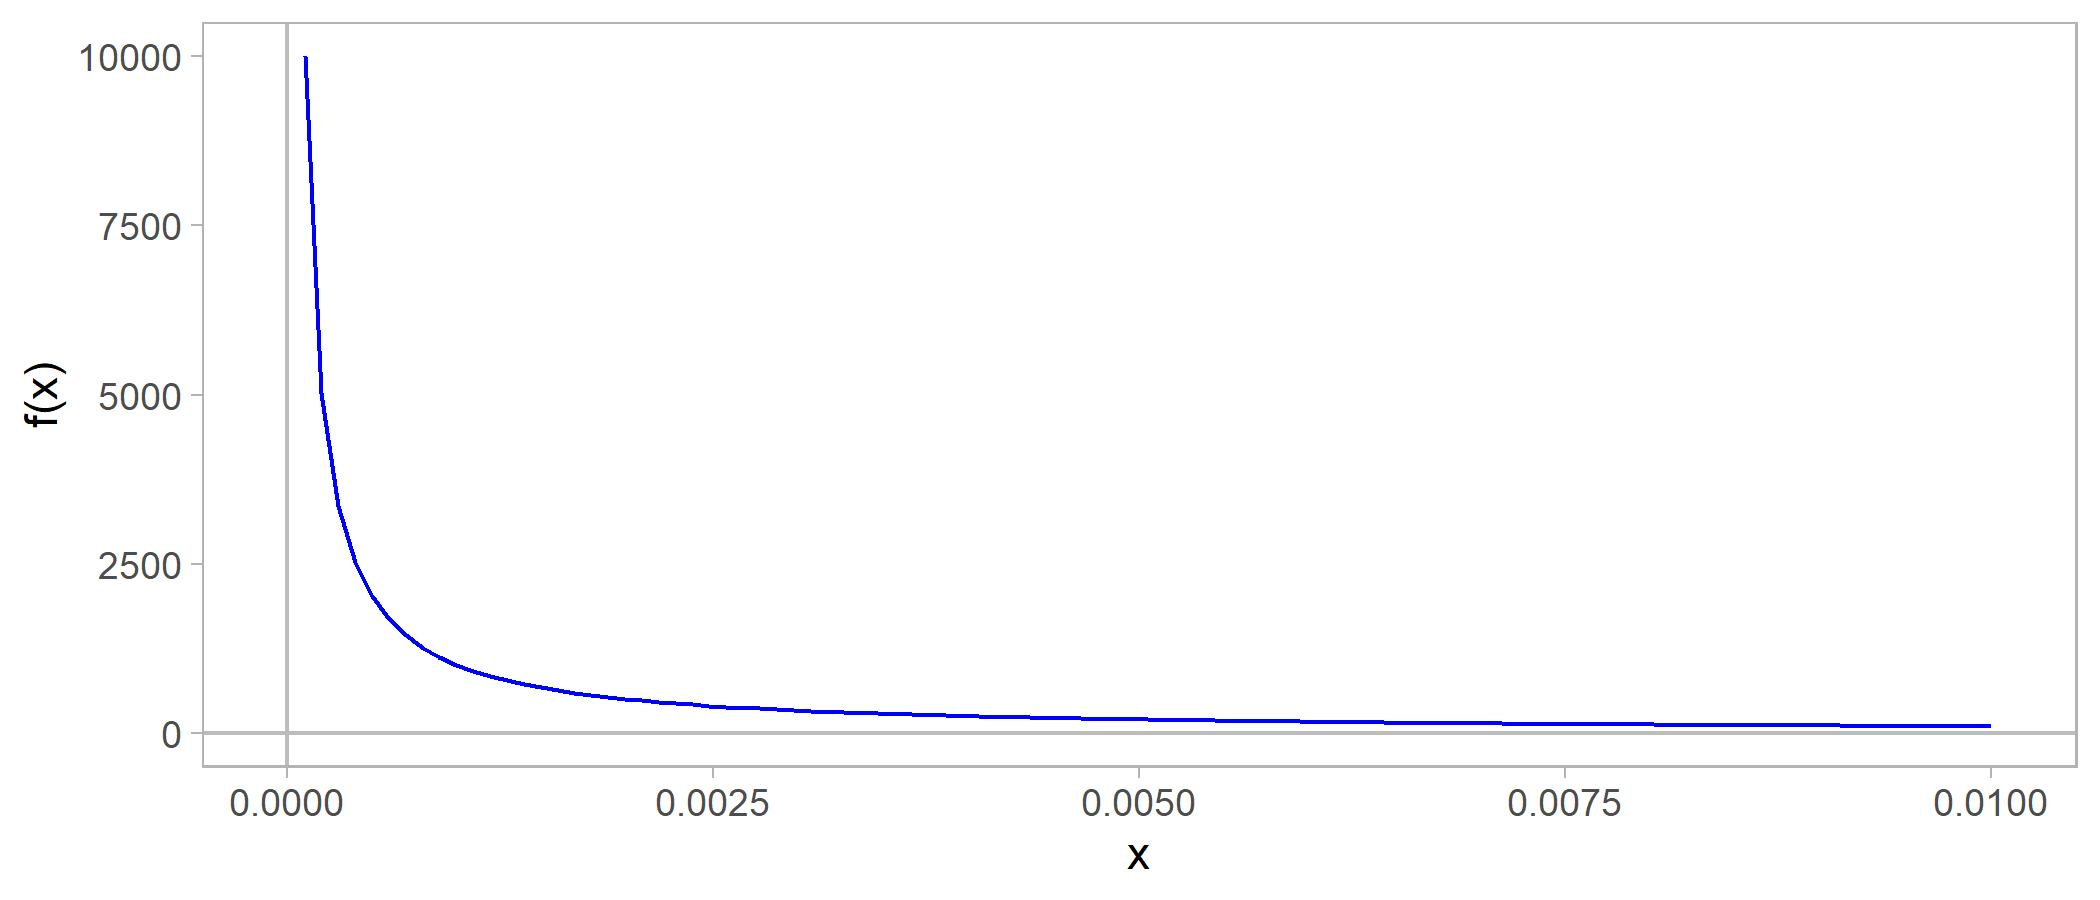
\includegraphics[scale=0.7]{img/infinite_limit_plot.jpg}
\end{figure}

Como podemos observar, a medida que $x \to 0^{+}$, $f(x)$ se va haciendo asíntota al eje $Y$; y cuando el límite se comporta de esta manera, vamos a decir que es igual al \textbf{\underline{infinito positivo}}.
\[\lim_{x \to 0^{+}} \frac{1}{x} = + \infty\]
En otras palabras, lo que estamos diciendo es, a medida que $x \to 0^{+}$, \textbf{el límite no existe \underline{porque} comienza a aumentar cada vez más hacia el infinito positivo}. En el caso en que otra función se mueva sin parar hacia la otra dirección (en este caso, hacia abajo), diremos que el límite no existe porque se mueve hacia \textbf{\underline{el infinito negativo}}.

Como ya hemos dicho, la ley del cuociente no nos dice mucho sobre el motivo por el que un límite no existe. Veamos los siguientes límites generales.
\[\lim_{x \to 0} \frac{1}{x} \, y \, \lim_{x \to 0} \frac{1}{x^{2}}\]
Ambos límites no existen, ya que nos encontramos con el ``Caso 2'' ($1/0$), no obstante, otra vez no sabemos por qué no existen. ¿Se comportan de la misma manera? Si no, entonces ¿por qué no existen? Averigüémoslo.

Digamos que $f(x) = 1/x$ y $g(x) = 1/x^{2}$. Construyamos una tabla para ambas funciones, tomando valores en donde $x \to 0$ desde la izquierda como de la derecha.

\begin{table}[hbt!]
\centering

\begin{tabular}{c | c | c}
$x$ & $f(x)$ & $g(x)$\\
\hline
-0.0001 & -10000 & 100000000\\
-0.001 & -1000 & 1000000\\
-0.005 & -200 & 40000\\
-0.01 & -100 & 10000\\
0.01 & 100 & 10000\\
0.005 & 200 & 40000\\
0.001 & 1000 & 1000000\\
0.0001 & 10000 & 100000000\\
\end{tabular}

\end{table}

Como ya podemos ver, pareciera que cuando $x \to 0^{-}$ la función $1/x$ viaja hacia el infinito negativo probablemente siendo asintota al eje $Y$, mientras que $1/x^{2}$ se mueve hacia el infinito positivo tanto vinendo los valores desde la izquierda como desde la derecha de cero. Comprobemos gráficamente aquello.

\begin{figure}[hbt!]
\centering
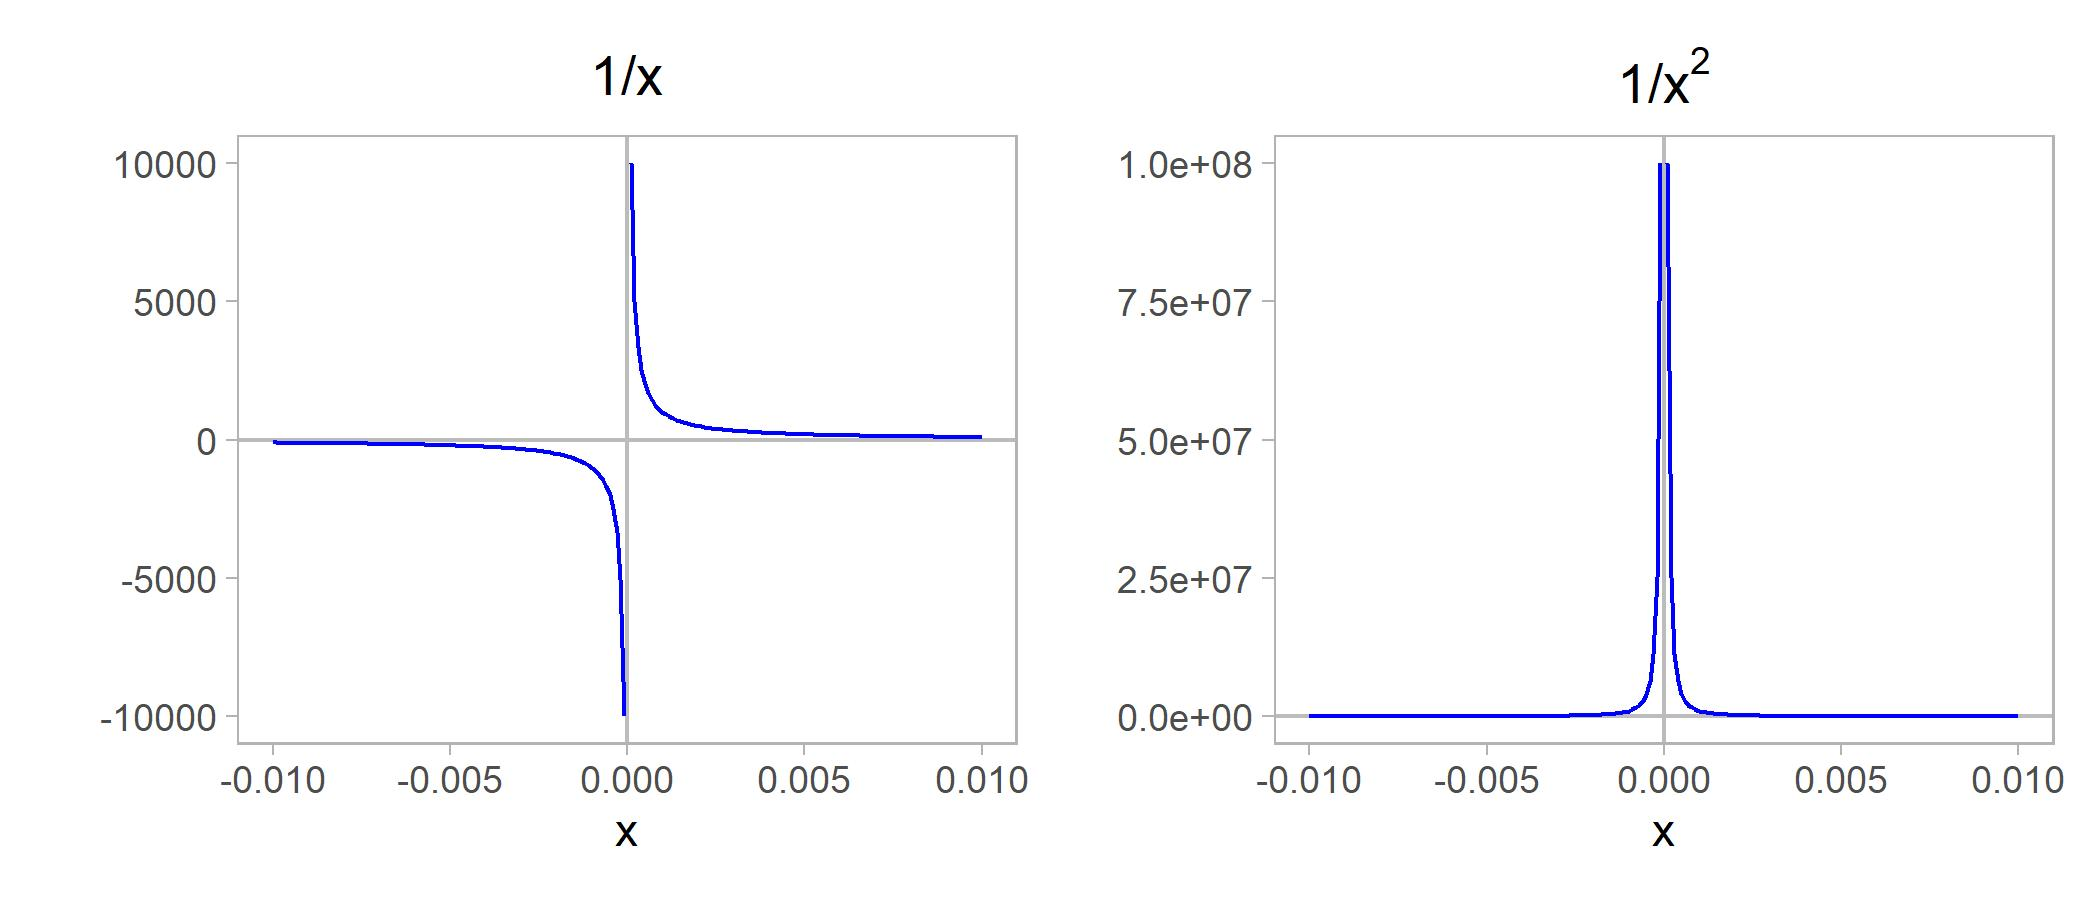
\includegraphics[scale=0.7]{img/infinite_limit_plot_2.jpg}
\end{figure}

\newpage

En definitiva, tanto el $\lim_{x \to 0} 1/x$ como el $\lim_{x \to 0} 1/x^{2}$, no existen, pero el primero es porque cuando $x \to 0^{-}$ la función va al infinito negativo, mientras que cuando $x \to 0^{+}$ la función va al infinito positivo. En cuanto al segundo límite, en ambos casos éste va al infinito positivo, siendo asíntotas al eje $Y$.

Ahora veamos el límite de una función más compleja:
\[\lim_{x \to 2}\left[\frac{3x}{4 - x^{2}}\right]\]
Tanto la función del numerador como del denominador, son continuas, por lo que:
\[\lim_{x \to 2}\left[\frac{3x}{4 - x^{2}}\right] = \frac{3(2)}{4 - (2)^{2}}\]
\[\lim_{x \to 2}\left[\frac{3x}{4 - x^{2}}\right] = \frac{6}{0}\]
De manera que este límite \textbf{no existe} (``Caso 2'').

Por otra parte, si graficamos aquella función, es probable que encontremos una asíntota en $x = 2$, pero no sabemos si la función irá al infinito positivo, al negativo o si se comporta de una manera totalmente distinta. Para tratar ésto, una forma más fácil es ver el límite separadamente, es decir, cuando $x \to 2^{-}$ y $x \to 2^{+}$.

Partamos con el límite de la función cuando $x \to 2^{-}$.

Cuando $x \to 2^{-}$, el numerador $3x \approx 6$ (es decir, un número positivo), mientras que el denominador $4 - x^{2} \approx 0$, pero ¿qué tan cerca de cero?

En este caso, $x \to 2^{-}$, $x$ va a ser \underline{ligeramente menor} a 2:
\[x < 2\]
Lo cual quiere decir que $x^{2}$ va a ser \underline{ligeramente menor} a 4:
\[x^{2} < 4\]
Por consiguiente, el denominador va a ser solo \underline{un poco mayor} a cero:
\[4 - x^{2} > 0\]
En otras palabras, el denominador $4 - x^{2}$ va a ser un número muy cercano a cero (mayor a éste), pero \underline{positivo}. De manera que el cuociente de la función cuando $x \to 2^{-}$, va a ser un valor positivo muy grande. En consecuencia:
\[\lim_{x \to 2^{-}}\left[\frac{3x}{4 - x^{2}}\right] = +\infty\]
Ahora veamos de la misma manera el límite de la derecha:
\[\lim_{x \to 2^{+}}\left[\frac{3x}{4 - x^{2}}\right]\]
A medida que $x \to 2^{+}$, también nuestro numerador $3x \approx 6$ y nuestro denominador $4 - x^{2} \approx 0$, pero esta vez estamos buscando valores de $x$ que sean \underline{ligeramente mayores} a 2:
\[x > 2\]
Lo que va a significar que $x^{2}$ va a ser \underline{ligeramente mayor} a 4:
\[x^{2} > 4\]
Por lo tanto, nuestro denominador $4 - x^{2}$ ahora va a ser \underline{un tanto menor} a cero:
\[4 - x^{2} < 0\]
En otras palabras, el denominador $4 - x^{2}$ va a ser un número negativo y, por consiguiente, el cuociente de la función va a ser un número grande otra vez, pero ahora será de signo negativo. Es decir, el límite de nuestra función cuando $x \to 2^{+}$, va a ser igual al \underline{infinito negativo}:
\[\lim_{x \to 2^{+}}\left[\frac{3x}{4 - x^{2}}\right] = - \infty\]

\newpage

Veamos ahora la gráfica de esta función tanto para cuando $x \to 2^{-}$ y para el caso de $x \to 2^{+}$. Para ser más ordenado, nombraremos a nuestra función como $h(x)$:
\[h(x) = \frac{3x}{4 - x^{2}}\]

\begin{figure}[hbt!]
\centering
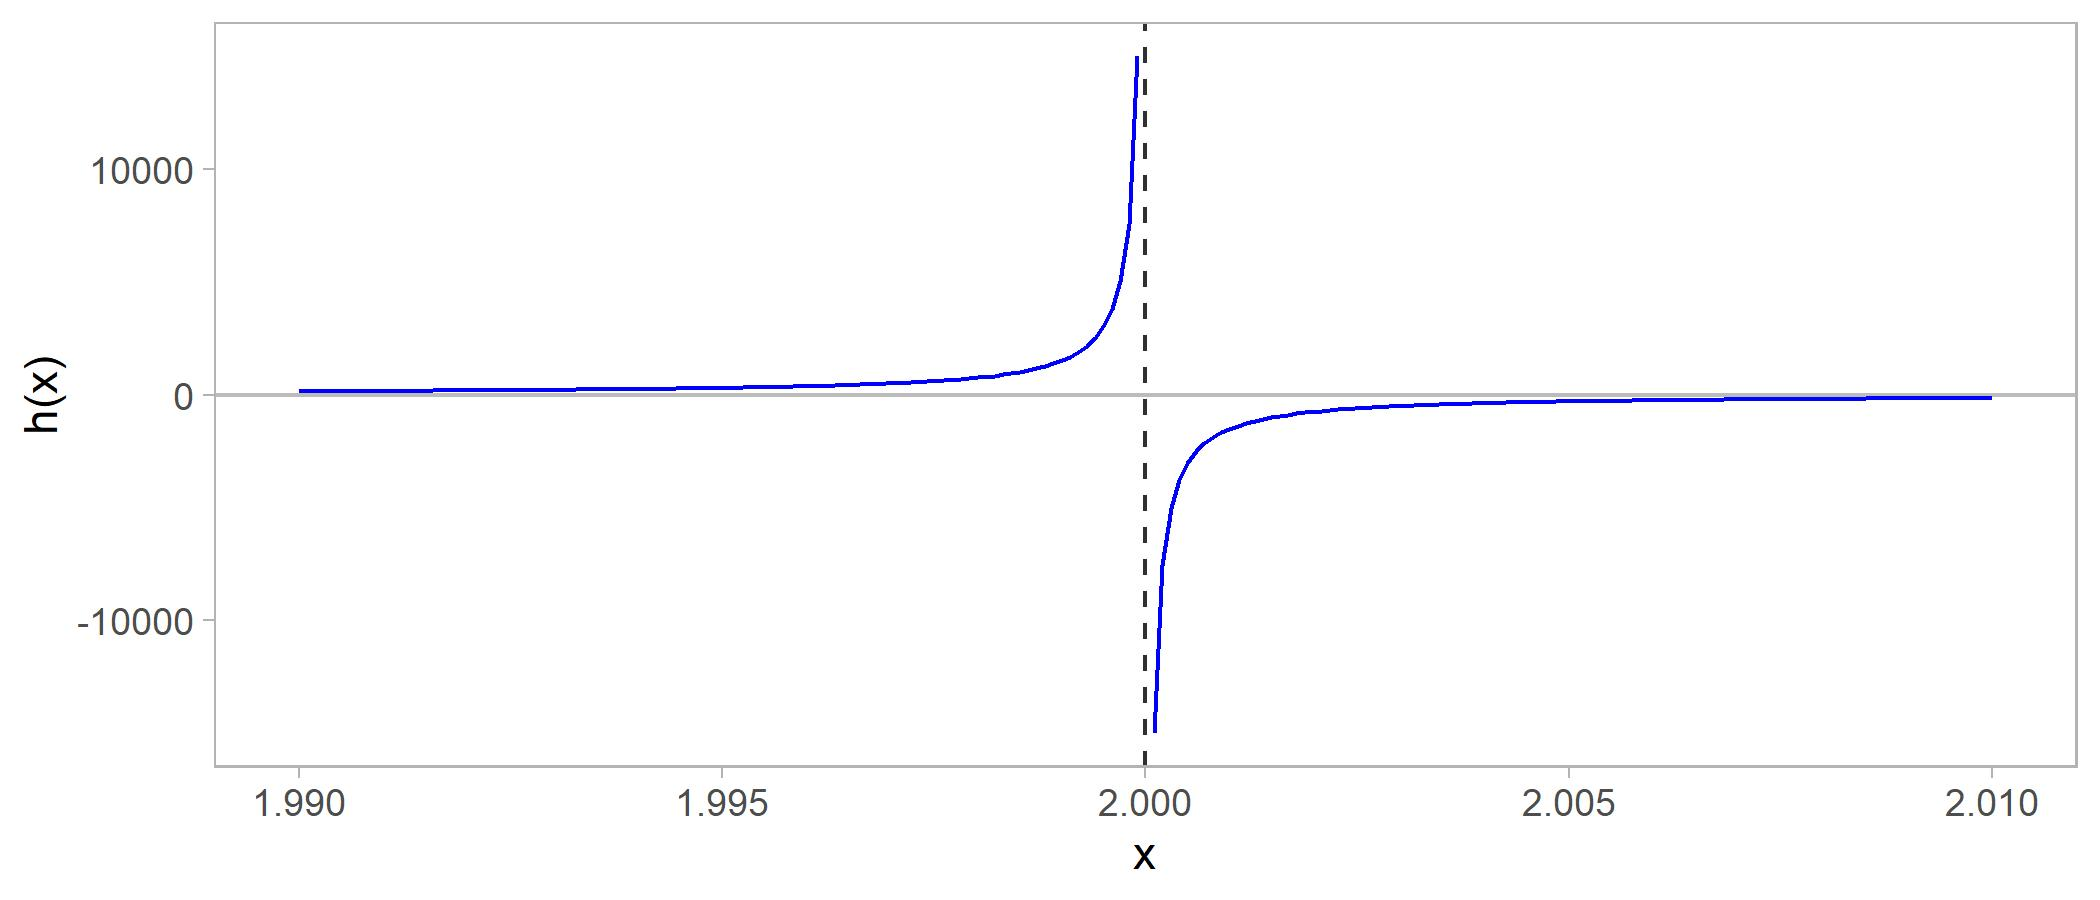
\includegraphics[scale=0.7]{img/infinite_limit_plot_3.jpg}
\end{figure}









































\end{document}